\chapter{Stato dell'arte}
\label{StatoArte}
\thispagestyle{empty}

%\begin{quotation}
%{\footnotesize
%\noindent{\emph{``Terence: Rotta a nord con circospezione \\
%Bud: Ehi, gli ordini li do io qui!\\
%Terence: Ok, comante\\
%Bud: Rotta a nord\\
%Terence: Soltanto?\\
%Bud: Con circospezione!''}
%}
%\begin{flushright}
%Chi Trova un Amico Trova un Tesoro
%\end{flushright}
%}
%\end{quotation}
\vspace{0.5cm}

\noindent In questo capitolo presentiamo i concetti fondamentali della teoria alla base della \textit{visione artificiale} e lo studio fatto finora sul problema del \textit{tampering detection}.
Nel primo paragrafo diamo una visione generale del modello della camera, senza pretendere una completa e dettagliata descrizione, bens\`i una visione pi\`u generale per comprendere meglio gli argomenti trattati nei capitoli successivi.
Nel secondo paragrafo descriviamo le soluzioni al problema del tampering detection presenti nella letteratura scientifica, definendo inoltre i concetti e la terminologia che verr\`a utilizzata nel resto della trattazione.
\section{Modello della camera}
Affinch\'e un sistema di visione artificiale possa risolvere il problema per cui \`e stato progettato, \`e necessario che esso sia in grado di acquisire una porzione della realt\`a che lo circonda.
Questo compito viene svolto da un particolare sensore chiamato \textit{camera}, il cui scopo principale \`e quello di creare una \textit{proiezione} dell'ambiente \textit{tridimensionale} in un sistema \textit{bidimensionale}.
Il principio alla base della camera \`e un concetto inventato da \textit{Filippo Brunelleschi} nel XV secolo, chiamato \textit{prospettiva a punto unico di fuga} (\textit{pinhole perspective}).
Il modello matematico utilizzato considera uno spazio tridimensionale, detto \textit{ambiente}, e un piano bidimensionale chiamato \textit{immagine}. 
I punti su tale piano sono la \textit{proiezione} dell'ambiente tridimensionale.
La proiezione \`e dovuta a un punto, chiamato \textit{centro ottico}, in cui viene convogliata la luce emanata dall'ambiente tridimensionale.
In questa astrazione, ciascun punto dello spazio tridimensionale viene associato univocamente a un punto nel piano immagine attraverso il raggio di luce che passa dal centro ottico.
\begin{figure}
	\centering
	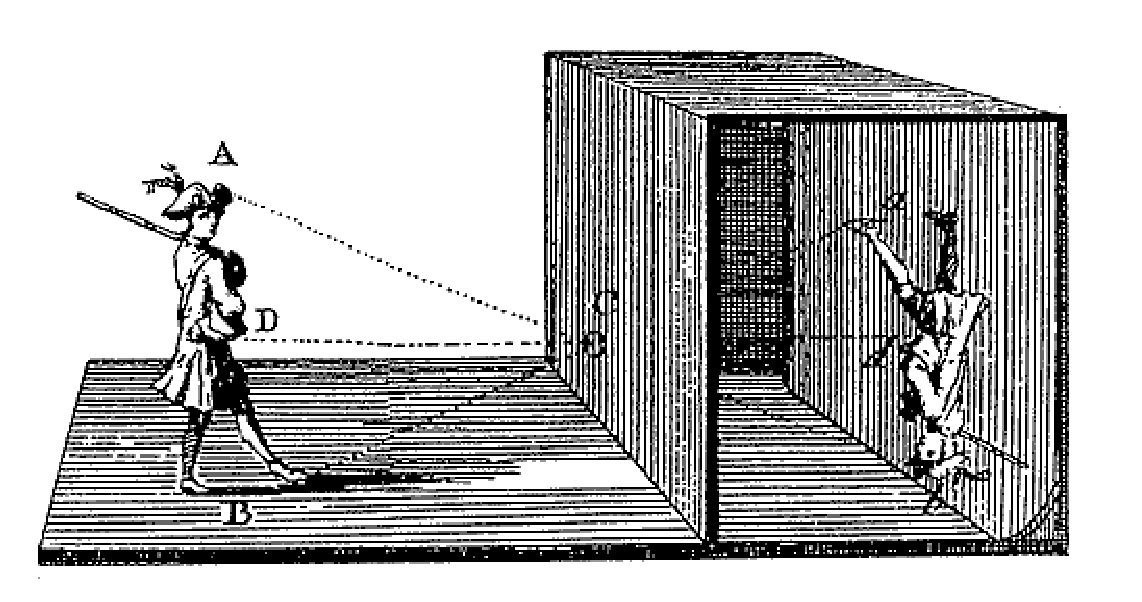
\includegraphics[width=12cm]{./pictures/cameraObscura}
	\caption{Athanasius Kircher, Principio della prospettiva nella camera obscura, 1671}
	\label{fig:prospettiva}
\end{figure} 
All'epoca di Brunelleschi, il modello del centro ottico veniva realizzato da una \textit{camera oscura}, come si pu\`o osservare nell'illustrazione in figura \ref{fig:prospettiva}, mentre nei moderni sistemi di acquisizione viene realizzato tramite \textit{lenti ottiche}. 
\subsection{La matrice prospettica della camera}
\begin{figure}
	\centering
	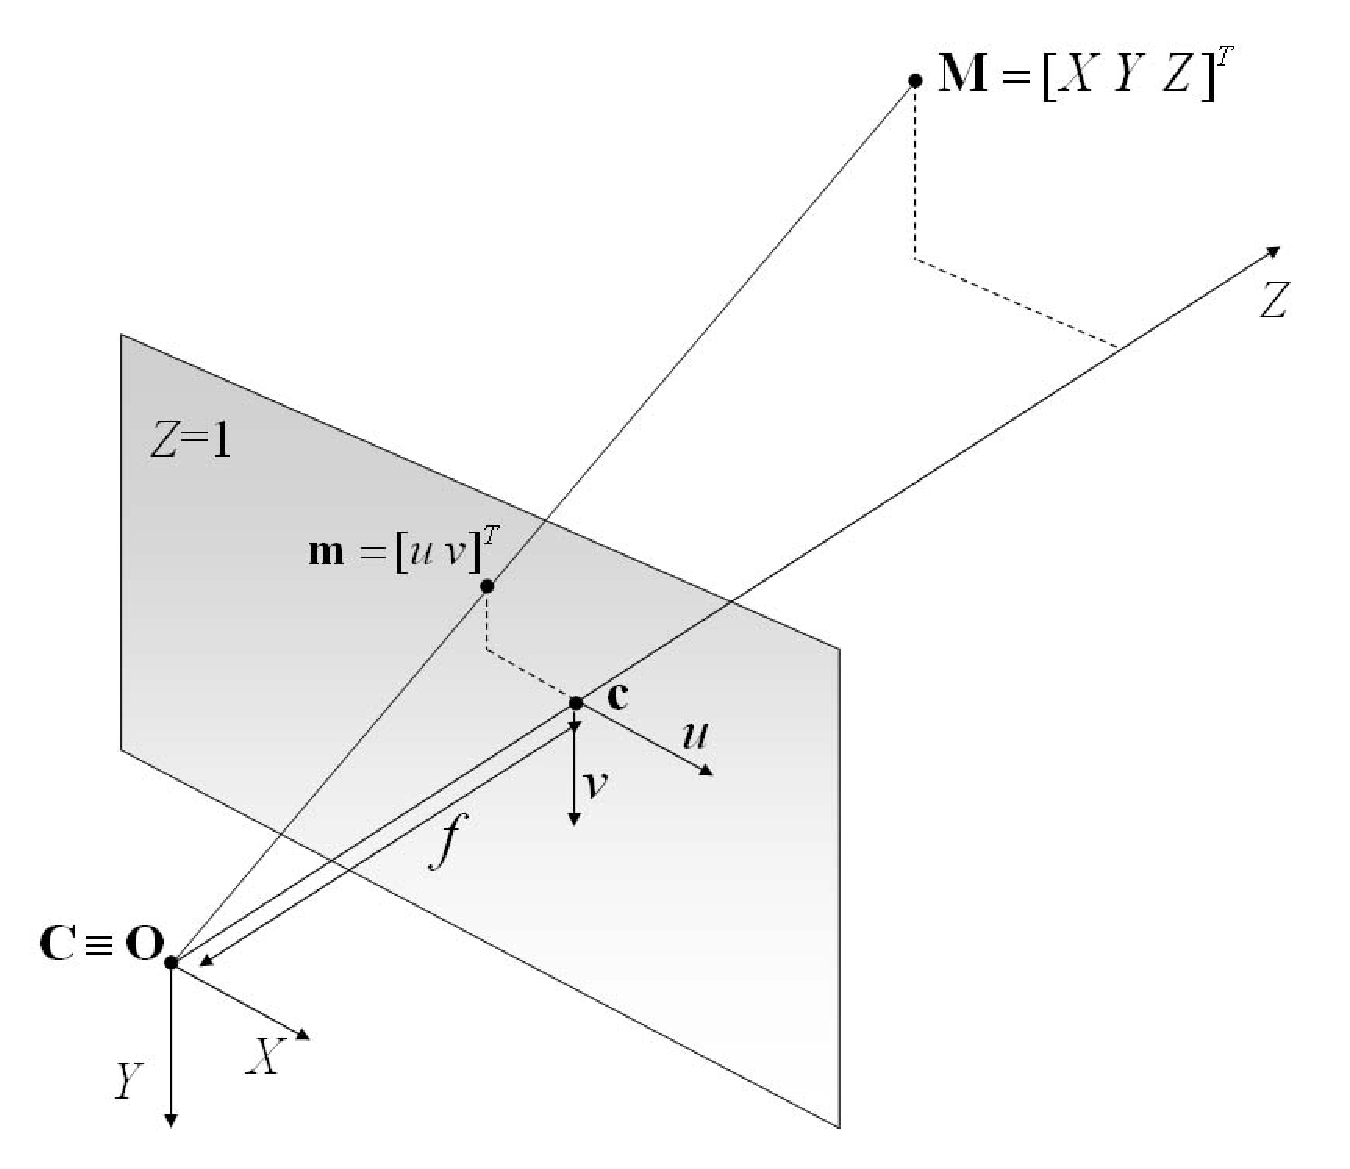
\includegraphics[width=10cm]{./pictures/modelloCamera}
	\caption{Schematizzazione del sistema ottico della camera}
	\label{fig:modelloCamera}
\end{figure} 
Nella figura \ref{fig:modelloCamera} sono illustrati i concetti che sono utilizzati per descrivere il sistema ottico della camera.
Indichiamo con $\textbf{M}=[X, Y, Z]^\textit{T}$ un qualsiasi punto nello spazio tridimensionale e con $\textbf{m} = [u, v]^\textit{T}$ la sua proiezione sul piano immagine dovuta al centro ottico $\textbf{C}$.
La linea che congiunge il centro ottico $\textbf{C}$ perpendicolarmente al piano immagine \`e detta \textit{asse principale}, indicata con $Z$, e il suo punto di intersezione con il piano stesso viene definita \textit{punto principale} $\textbf{c}$.
La distanza tra il punto principale e il centro ottico viene definita \textit{distanza focale},  e viene indicata con $f$.\\
La rappresentazione dei punti viene fatto attraverso le loro \textit{coordinate omogenee}.
In questo modo \`e possibile rappresentare le trasformazioni tra sistemi di coordinate di ordine differente tramite una singola trasformazione matriciale.
Chiamiamo coordinate omogenee di un punto $\textbf{m} = [u,v]$ del piano una qualsiasi terna ordinata $[U,V,W]$ di numeri reali tali che
\[W\neq 0,
\frac{U}{W}=u,
\frac{V}{W}=v.\]
Analogamente, le coordinate omogenee di un punto $\textbf{M}=[x,y,z]$ nello spazio tridimensionale saranno costituite da una quaterna di numeri $[X,Y,Z,W]$ tali che 
\[W\neq 0,
\frac{X}{W}=x,
\frac{Y}{W}=y,
\frac{Z}{W}=z.\]
La coordinata $W$ viene definita \textit{valore di scala}; nel caso $W=1$ le rimanenti coordinate omogenee rappresentano le \textit{coordinate cartesiane} del punto.\\
Consideriamo un punto $\textbf{M}$ nello spazio tridimensionale, rappresentato tramite le coordinate omogenee $[X,Y,Z,1]^\textit{T}$, e il suo punto immagine $\textbf{m}$ rappresentato dalle coordinate omogenee $[u,v,1]^\textit{T}$.
La proiezione della camera pu\`o essere espressa come
\begin{equation}
\label{eq:proiezione}
\textbf{m}=P\textbf{M},
\end{equation}
dove $P$  \`e una matrice di dimensioni $3 \times 4$ chiamata \textit{matrice prospettica} \cite{hartley2003multiple}.
Tale matrice contiene al suo interno informazioni sui parametri della camera a cui \`e associata, e descrive sia la proiezione sul piano immagine che le trasformazioni di camera rispetto al sistema di riferimento tridimensionale.
Formalmente viene rappresentata attraverso due matrici: una che rappresenta i \textit{parametri intrinseci} e un'altra che rappresenta i \textit{parametri estrinseci} \cite{forsyth2002computer}.
\begin{itemize}
	\item I \textit{parametri intrinseci} rappresentano le caratteristiche interne della camera come la distanza focale, il centro focale e le caratterisitiche di \textit{distorsione} della lente.
	\item I \textit{parametri estrinseci} rappresentano la posizione della camera rispetto al sistema di riferimento dello spazio tridimensionale.
\end{itemize} 
\subsection{Parametri intrinseci}
La relazione fra le coordinate tridimensionali di un punto $\textbf{M}=[X,Y,Z]$ e le coordinate del suo proiettato $\textbf{m}=[u,v]$ \`e:
\[u=f\cdot \frac{X}{Z},\]
\[v=f\cdot \frac{Y}{Z}.\]
\begin{figure}
	\centering
	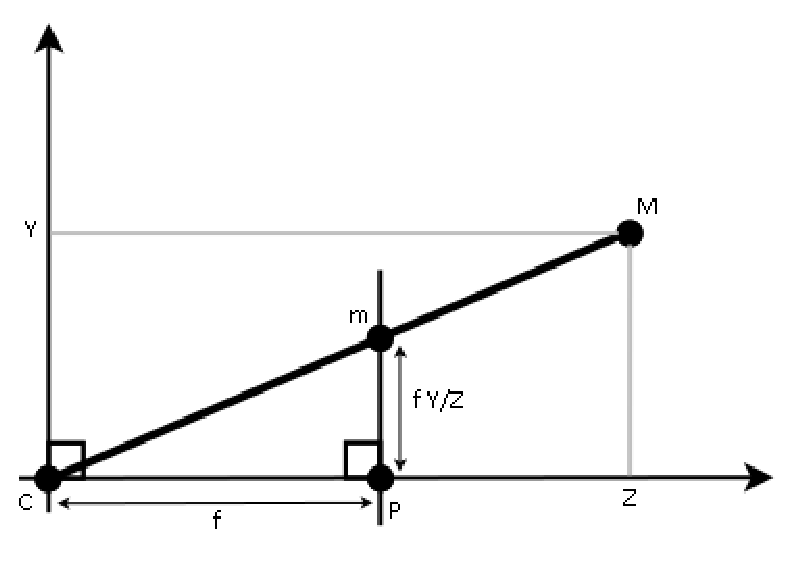
\includegraphics[width=10cm]{./pictures/mappatura2d3d}
	\caption{Similitudini tra triangoli usate nel calcolo dei parametri intrinseci}
	\label{fig:mapping}
\end{figure}
\noindent Tale relazione deriva dalle propriet\`a dei triangoli simili, come mostra la figura \ref{fig:mapping}.
La \textit{mappatura} viene definita, dunque, dalla seguente relazione:
\begin{equation}
\label{eq:mapping}
[X,Y,Z]^\textit{T} \mapsto \left[f\cdot \frac{X}{Z}, f\cdot \frac{Y}{Z}\right]^\textit{T}.
\end{equation} 
Se il punto nello spazio e il suo proiettato sono rappresentati attraverso le loro coordinate omogenee, la \eqref{eq:mapping} pu\`o essere riscritta come
\begin{equation}
\label{eq:mappingMatrix}
\left[\begin{array}{c}
X \\ Y \\ Z \\ 1
\end{array}\right] \mapsto 
\left[\begin{array}{c}
fX \\ fY \\ Z
\end{array}\right] = 
K \left[\begin{array}{rcl}
I & | & 0
\end{array}\right]
\left[\begin{array}{c}
X \\ Y \\ Z \\ 1
\end{array}\right],
\end{equation}
dove la matrice
\begin{equation}
\label{eq:kSimple}
K = 
\left[\begin{array}{rccl}
f & & \\
& f & \\
& & 1 
\end{array}\right]
\end{equation}

viene detta \textit{matrice di calibrazione} della camera.\\
Nella formula \eqref{eq:mapping} abbiamo assunto che l'origine delle coordinate del piano immagine si trovi nel punto principale, come \`e illustrato nella figura \ref{fig:modelloCamera}.
Se consideriamo il punto principale di coordinate $[p_u, p_v]$, la \eqref{eq:mapping} diventa
 \begin{equation}
 \label{eq:mappingGeneral}
 [X,Y,Z]^\textit{T} \mapsto \left[f\cdot \frac{X}{Z}+p_u, f\cdot \frac{Y}{Z}+p_v\right]^\textit{T},
 \end{equation}
 mentre la matrice di calibrazione\eqref{eq:kSimple} diventa 
 \begin{equation}
 \label{eq:kGeneral}
 K =
  \left[\begin{array}{rcl}
  f & & p_u \\
  & f & p_v \\
  & & 1 
  \end{array}\right].
 \end{equation}
 Nel caso in cui il sensore della camera sia \textit{digitale}, l'immagine deve essere quantizzata come una matrice di $W$ colonne e $H$ righe, in cui ciascun elemento prende il nome di \textit{pixel} (dalla contrazione di \textit{picture element}).
 \begin{figure}
 	\centering
 	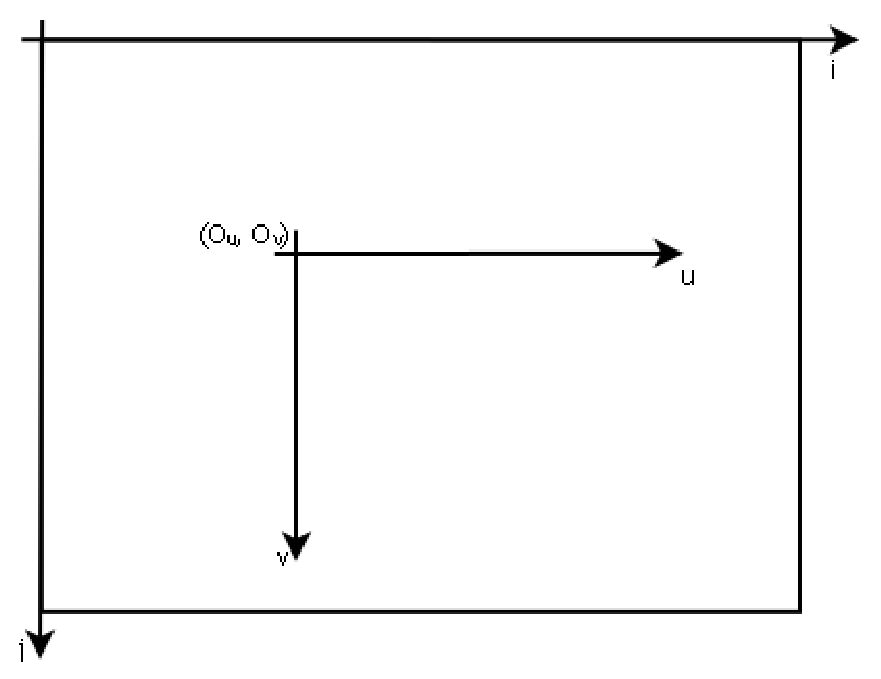
\includegraphics[width=8cm]{./pictures/griglia}
 	\caption{Coordinate di un frame}
 	\label{fig:griglia}
 \end{figure}
 Ogni pixel possiede, quindi, delle coordinate che definiscono la sua posizione sulla matrice del frame.
 Se definiamo con $(i,j)$ le coordinate del generico pixel sulla matrice del frame, dove l'origine \`e posta nell'angolo in alto a sinistra, e con $(O_u, O_v)$ le coordinate del punto principale secondo il sistema di riferimento del frame (si veda a riguardo la figura \ref{fig:griglia}), possiamo mettere in relazione le coordinate dell'immagine con le coordinate frame nel seguente modo:
 \[ u = (i - O_u) \cdot S_u \]
 e
 \[ v = (j - O_v) \cdot S_v, \]
 dove $S_u$ e $S_v$ sono le dimensioni orizzontali e verticali del singolo pixel.
 \`E necessario introdurre, nella matrice di calibrazione, l'informazione del numero di pixel per unit\`a di distanza in coordinate immagine $m_u$ e $m_v$, rispettivamente nelle direzioni $u$ e $v$, modificando la matrice di calibrazione definita in \eqref{eq:kGeneral} come
 \begin{equation}
 \label{eq:kDigital}
 K =
 \left[\begin{array}{rccl}
 \alpha_u & & u_0\\
 & \alpha_v & v_0\\
 & & 1
 \end{array}\right],
 \end{equation}
 dove $\alpha_u = fm_u$ e $\alpha_v=fm_v$, mentre il punto principale $[p_u, p_v]$ viene riscritto come $[u_0, v_0] = [m_u p_u, m_v p_v]$. \\
 Nel caso in cui la matrice di calibrazione sia nota, la camera viene detta \textit{completamente calibrata}.\\
 La matrice di calibrazione $K$ rappresenta, quindi, il cambio di sistema di riferimento nel piano immagine, ridefinendo il centro della camera $(u_0, v_0)$ in modo che coincida con il punto principale.
 \subsection{Parametri estrinseci}
 La matrice $K$ descritta dall'equazione \eqref{eq:kDigital} \`e valida per camere poste all'origine del sistema di riferimento.
Se consideriamo camere localizzate in una posizione arbitraria, quindi, \`e necessario che le coordinate dei punti, definite nel sistema di riferimento tridimensionale, siano ridefinite secondo il sistema di coordinate della camera.
 \begin{figure}
 	\centering
 	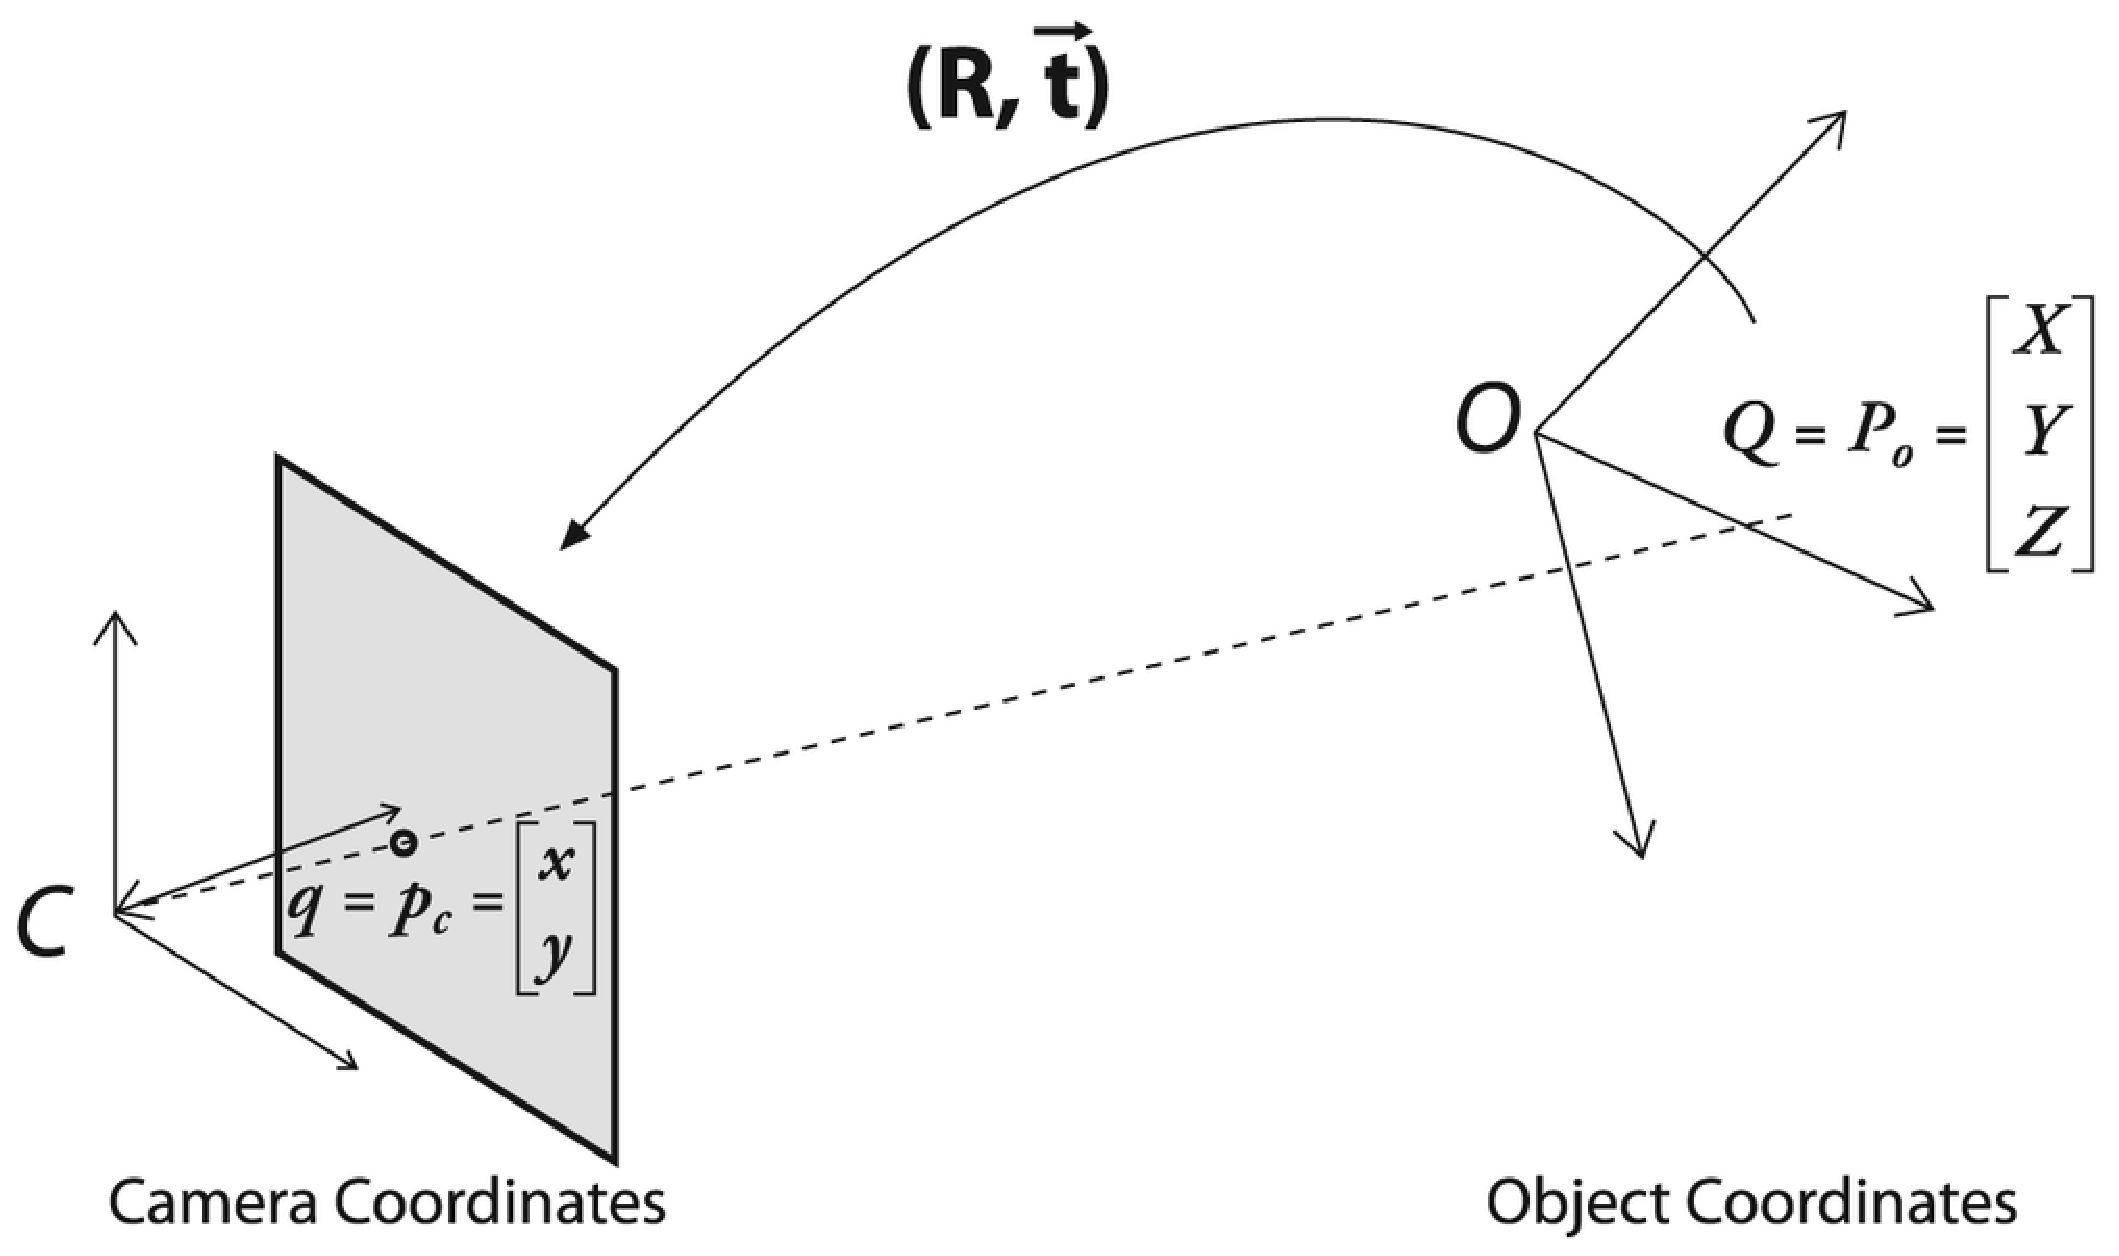
\includegraphics[width=8cm]{./pictures/rt}
 	\caption{Trasformazione dal sistema di coordinate dell'ambiente a quello della camera}
 	\label{fig:rt}
 \end{figure}
Questa trasformazione viene definita attraverso una \textit{rototraslazione}, nello spazio, del sistema di riferimento dell'ambiente, in modo che coincida con quello della camera.
Se $\tilde{\textbf{M}}$ rappresenta le coordinate cartesiane di un punto nel sistema di riferimento dell'ambiente e $\tilde{\textbf{M}}_{cam}$ rappresenta lo stesso punto nel sistema di riferimento della camera, si pu\`o scrivere
\begin{equation}
\label{eq:rototrals1}
\tilde{\textbf{M}}_{cam}=R(\tilde{\textbf{M}} - C),
\end{equation}
dove $C$ rappresenta le coordinate del centro della camera nel sistema di riferimento dell'ambiente, $R$ \`e una \textit{matrice di rotazione} $3 \times 3$ che rappresenta l'orientamento della camera rispetto al sistema di riferimento dell'ambiente e $K$ \`e la matrice di calibrazione della camera.
L'equazione \eqref{eq:rototrals1} pu\`o essere riscritta in forma matriciale: se definiamo $\textbf{M}$ e $\textbf{M}_{cam}$ come le rappresentazioni in coordinate omogenee di $\tilde{\textbf{M}}$ e $\tilde{\textbf{M}}_{cam}$, abbiamo
\[ \textbf{M}_{cam} =  \left[\begin{array}{cc}
R & -RC \\
0 & 1
\end{array}\right] 
\textbf{M}, \]
da cui, riprendendo l'equazione \ref{eq:mappingMatrix},
\begin{eqnarray}
\textbf{m} & = & K \left[\begin{array}{rcl}
I & | & 0
\end{array}\right]\textbf{M}_{cam} \nonumber \\
 & = & K \left[\begin{array}{rcl}
I & | & 0
\end{array}\right] 
\left[\begin{array}{cc}
R & -RC\\
0 & 1 
\end{array}\right] \textbf{M} \nonumber \\
 & = &
K \left[\begin{array}{rcl}
R & | & -RC
\end{array}\right]\textbf{M}. \nonumber
\end{eqnarray}
Possiamo, quindi, scrivere l'equazione della matrice di proiezione della camera come
\[P=K \left[\begin{array}{rcl}
R & | & t
\end{array}\right],\]
dove $t = -RC$ prende il nome di \textit{vettore di traslazione}.
%\section{Monitoraggio video: concetti e terminologia}
%Prima di concentrarci sul problema del tampering detection, definiamo, i concetti e i termini che verranno utilizzati nel seguito della trattazione.\\
%Lo scenario che consideriamo \`e quello di una camera che deve riprendere una particolare \textit{\gls{scena}}.
%\begin{figure}
%	\centering
%	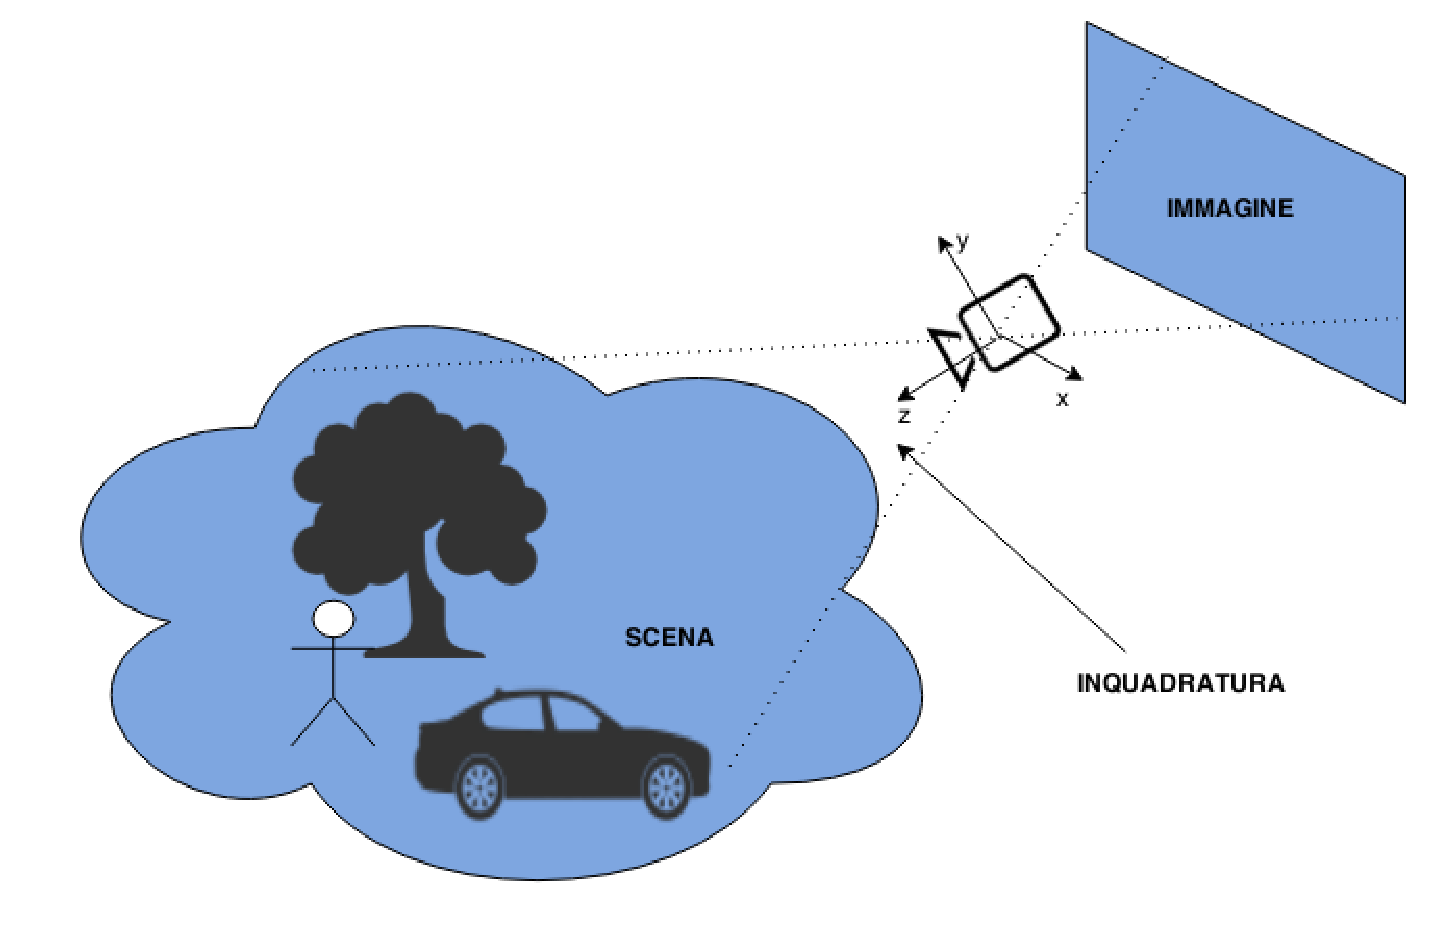
\includegraphics[width=12cm]{./pictures/videoMonitoring}
%	\caption{Sistema di monitoraggio video}
%	\label{fig:videoMonitoring}
%\end{figure}
%\noindent 
%La posizione e l'orientamento della camera determinano l'\textit{\gls{inquadratura}} della scena.
%L'acquisizione, da parte della camera, della scena nell'istante di tempo $i$ viene definita \textit{immagine} o \textit{frame} i-esimo.
%La figura \ref{fig:videoMonitoring} illustra questi concetti.\\
%Per semplificare l'analisi, considereremo immagini estratte in \textit{scala di grigi}.
%Quindi ciascuna immagine verr\`a rappresentata come una matrice di pixel, in cui ciascun elemento rappresenta l'intensit\`a luminosa (\textit{luma}) del pixel corrispondente.\\
%Nel seguito della trattazione useremo una specifica terminologia.
%Indicheremo con $\mathcal{X}$ l'insieme dei \textit{pixel} costituenti l'immagine acquisita dalla camera,
%\[ \mathcal{X} \subset \mathbb{N}^2, \]
%e con $x \in \mathcal{X}$ il singolo pixel.
%Quando vorremo considerare il frame acquisito all'istante di tempo $i$, useremo $z_i$, con $i=1,\dots , \infty$. 
%In particolare, per indicare il valore della \textit{luminosit\`a} del pixel $x$ per il frame $i$-esimo, useremo il termine $z_i(x)$, con 
%\[ z_i(x) \in [0, 255]. \]
\section{Tampering Detection}
Nei moderni sistemi di videosorveglianza troviamo spesso algoritmi utilizzati per identificare particolari eventi all'interno della scena ripresa dalla camera. 
Ad esempio \`e possibile avere un software in grado di identificare le targhe delle automobili che superano il limite di velocit\`a, oppure la presenza di oggetti incustoditi in una stazione \cite{Targhe}.
Affinch\'e questi algoritmi funzionino correttamente, \`e importante che l'\textit{affidabilit\`a} del sistema di acquisizione sia preservata.
Questa propriet\`a viene soddisfatta quando:
\begin{itemize}
	\item la camera mantiene la stessa inquadratura nel tempo;
	\item tutti gli elementi della scena sono presenti nell'immagine in maniera \textit{nitida}.
\end{itemize}
%In un'applicazione di monitoraggio video consideriamo che la camera, in condizioni di funzionamento ottimale, mantenga la stessa inquadratura nel tempo e che sia in grado di acquisire, in maniera nitida, tutti gli elementi di interesse presenti nella scena.
Definiamo \gls{tampering} un qualsiasi evento che determini un cambio di inquadratura o che non permetta la corretta acquisizione di una parte o della totalit\`a della scena.
Possiamo classificare gli eventi di tampering in quattro categorie:
\begin{itemize}
	\item sfocature,
	\item spostamenti della camera,
	\item occlusioni dell'obiettivo,
	\item guasti della camera.
\end{itemize}

Per affrontare il problema dell'identificazione di questo tipo di eventi, la letteratura scientifica offre molte tecniche che permettano l'identificazione automatica di eventi in grado di compromettere la corretta ripresa della scena da parte della videocamera.
\begin{figure}
	\centering
	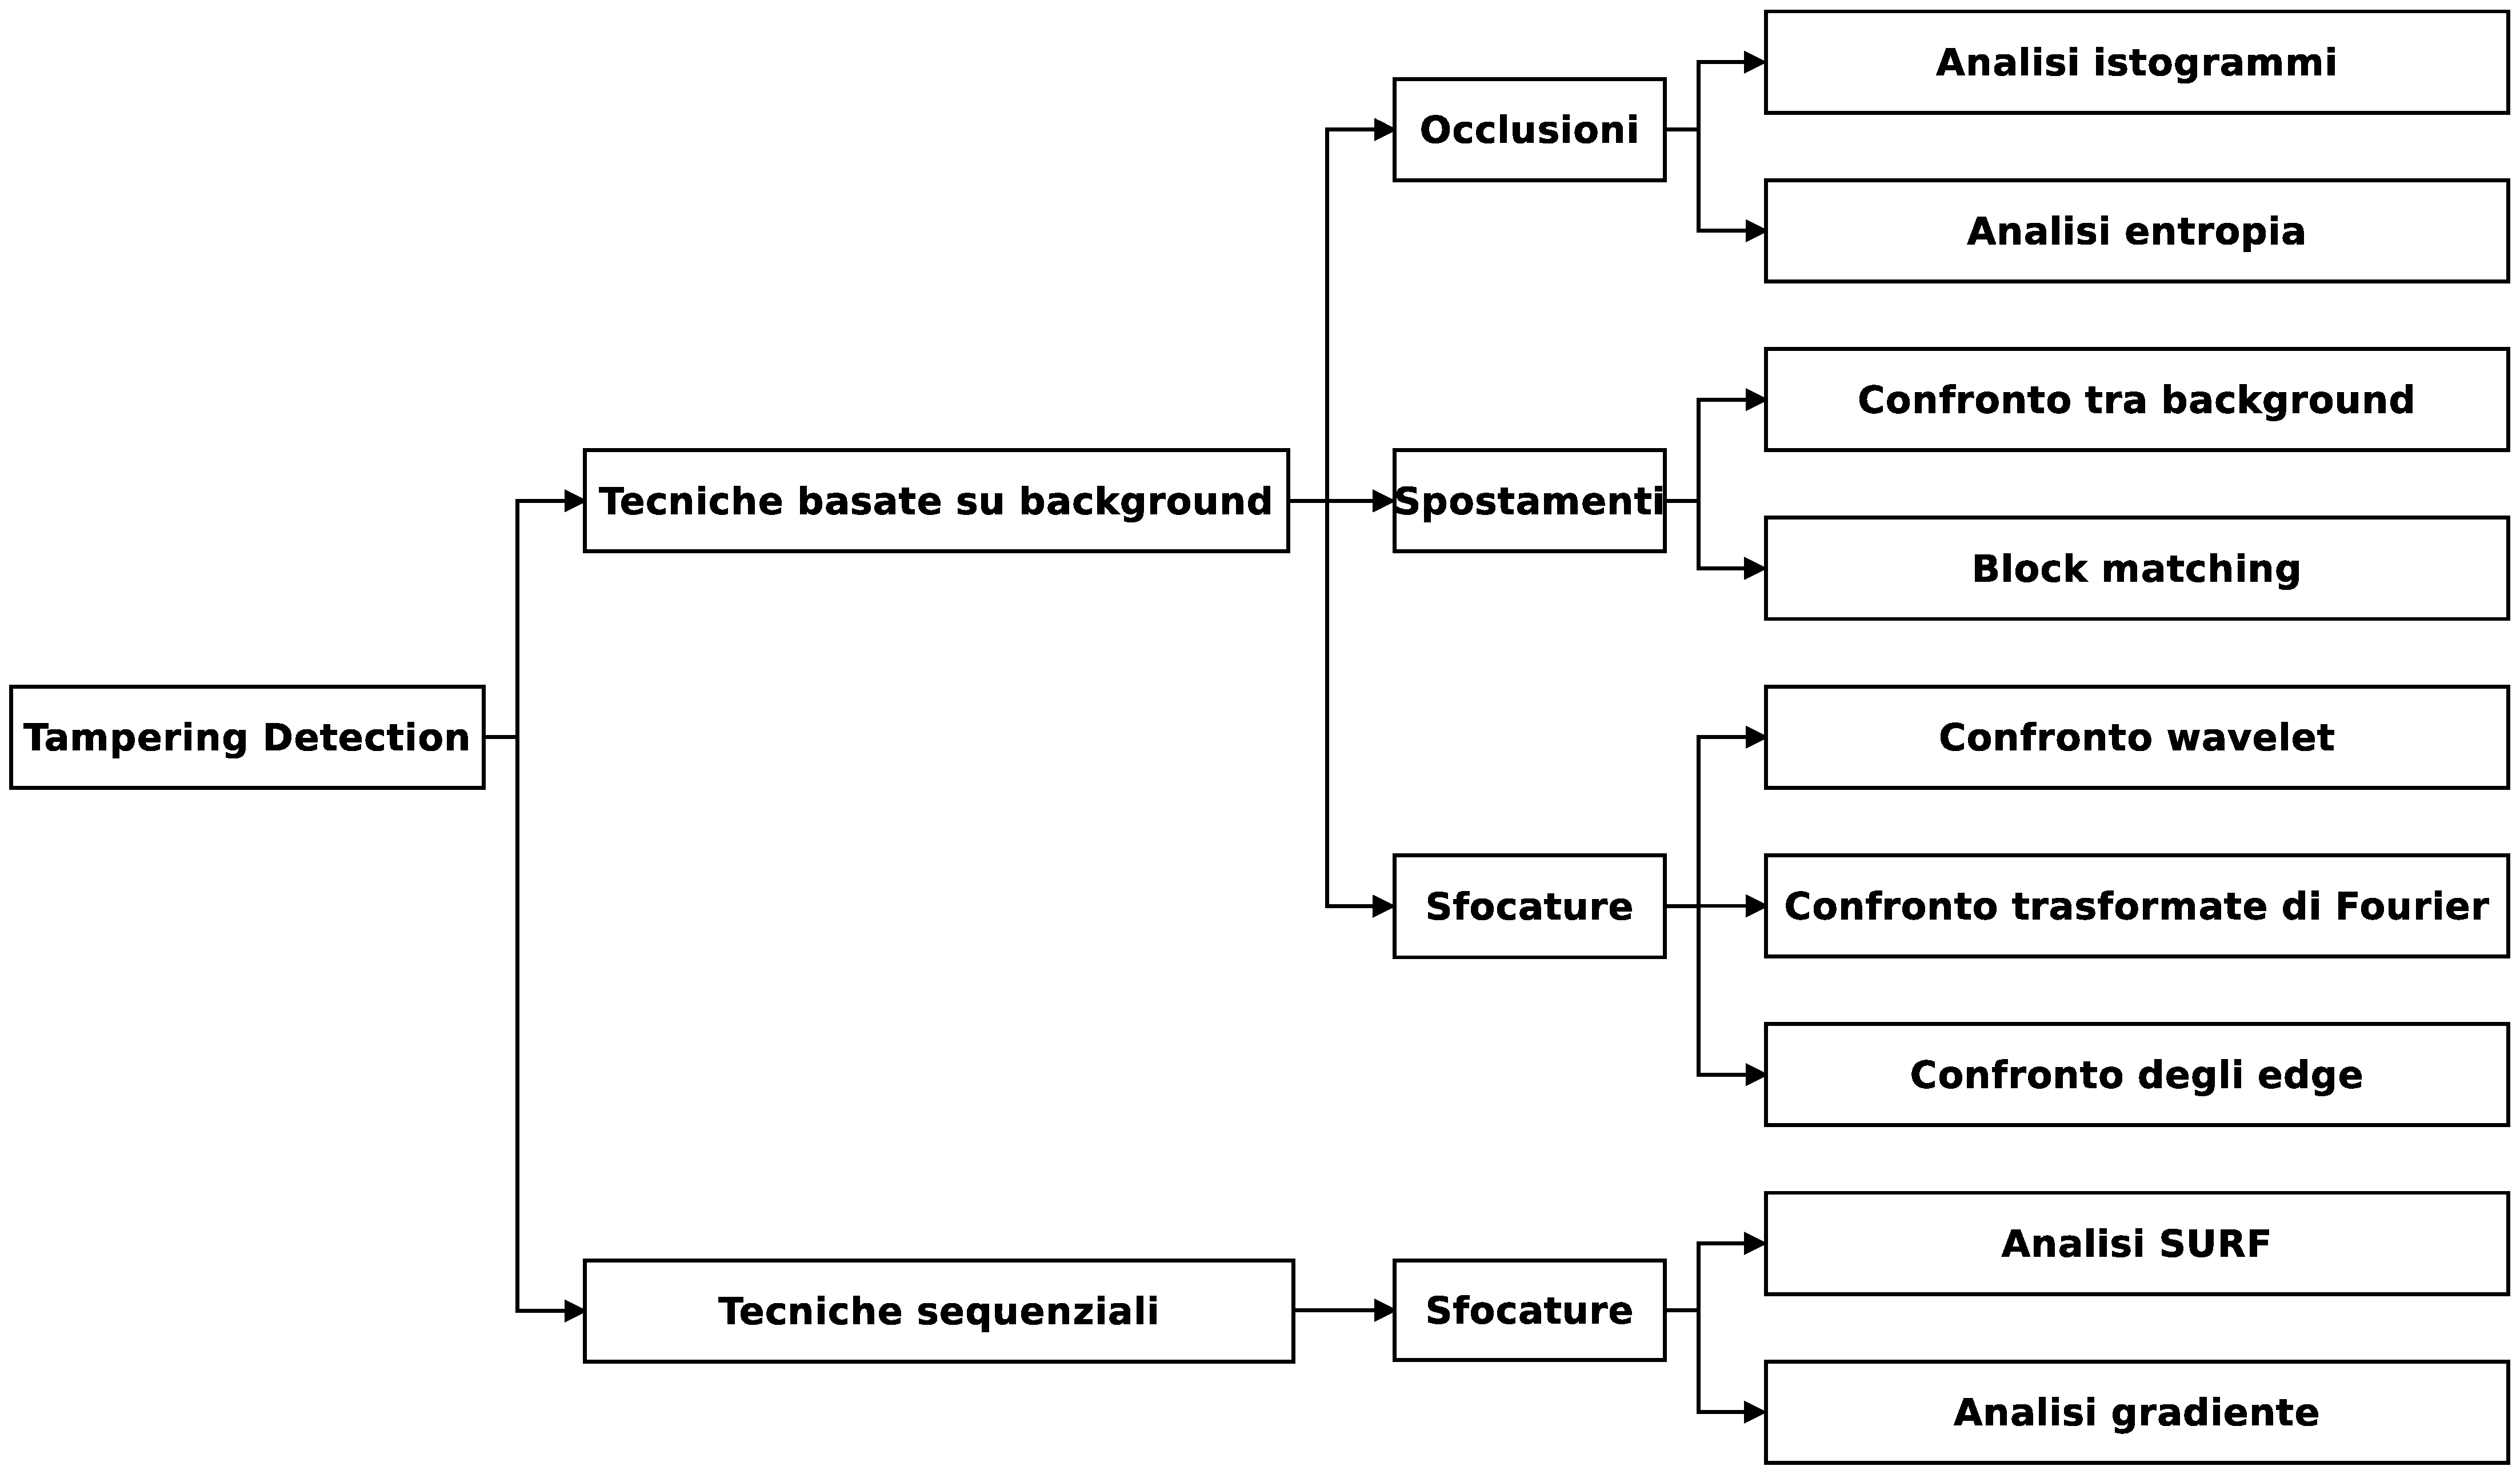
\includegraphics[width=12cm]{./diagrammi/tecnicheSOA.eps}
	\caption{Tecniche di tampering detection}
	\label{fig:tamperingSOA}
\end{figure}
Lo schema in figura \ref{fig:tamperingSOA} mostra le principali tecniche di tampering detection presenti in letteratura.
Queste possono essere divise in due categorie: 
\begin{itemize}
	\item tecniche basate su confronto di background,
	\item tecniche basate su monitoraggio sequenziale.
\end{itemize}
Nel seguito del paragrafo verranno descritti i principali metodi utilizzati in queste due categorie.
\subsection{Concetti e terminologia}
Prima di concentrarci su come \`e stato affrontato il problema del tampering detection, definiamo i concetti e i termini che verranno utilizzati nel seguito della trattazione.\\
Lo scenario che consideriamo \`e quello di una camera che deve riprendere una particolare \textit{\gls{scena}}.
\begin{figure}
	\centering
	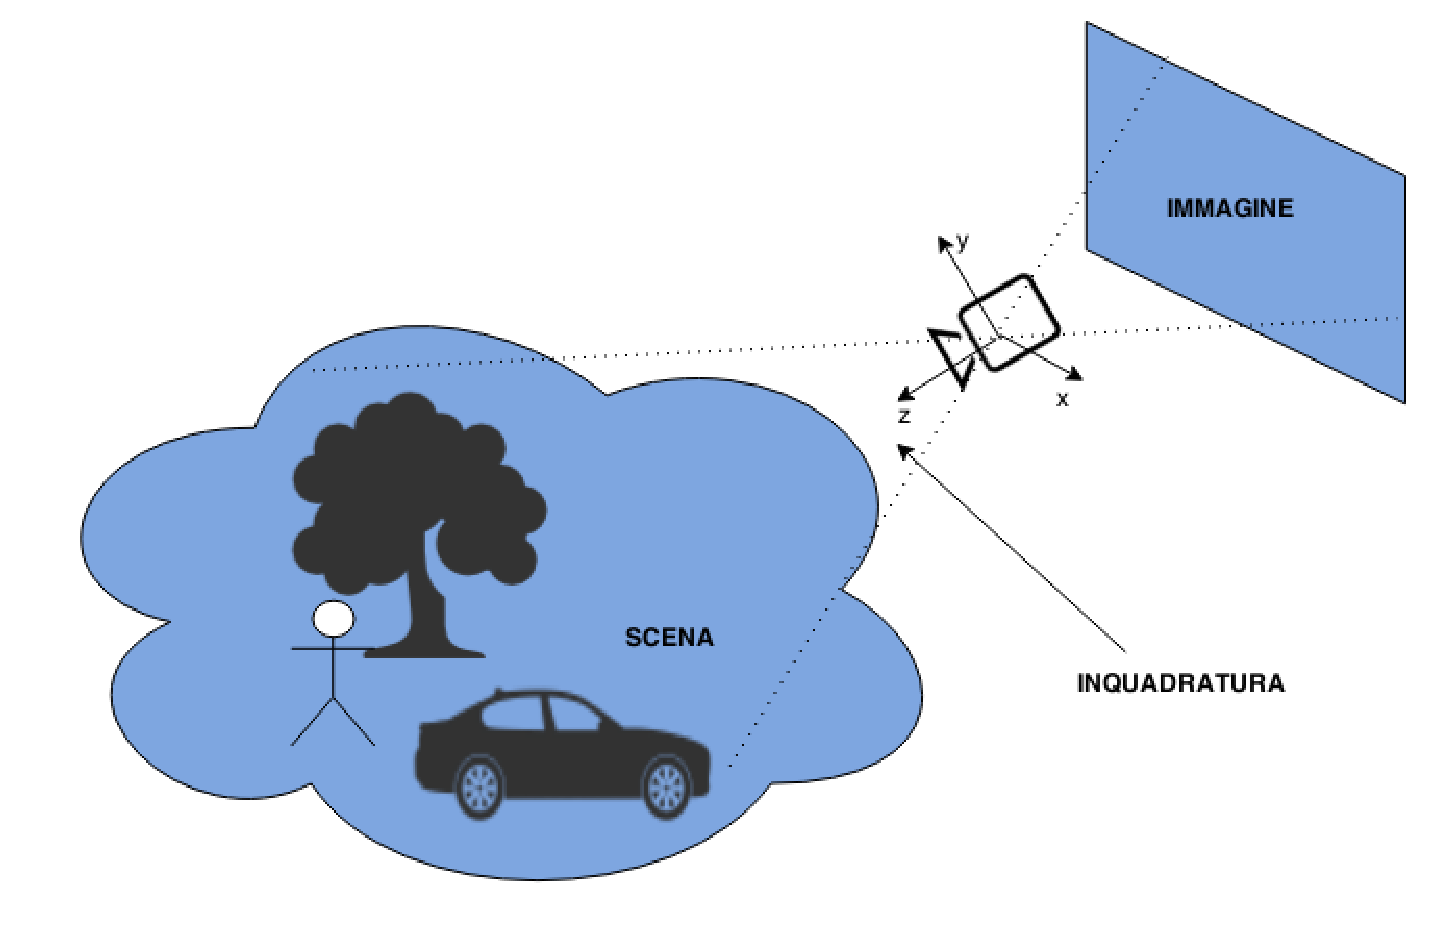
\includegraphics[width=12cm]{./pictures/videoMonitoring}
	\caption{Sistema di monitoraggio video}
	\label{fig:videoMonitoring}
\end{figure}
\noindent 
La posizione e l'orientamento della camera determinano l'\textit{\gls{inquadratura}} della scena.
L'acquisizione, da parte della camera, della scena nell'istante di tempo $i$ viene definita \textit{immagine} o \textit{frame} i-esimo.
La figura \ref{fig:videoMonitoring} illustra questi concetti.\\
Per semplificare l'analisi, considereremo immagini estratte in \textit{scala di grigi}.
Ciascuna immagine, quindi, verr\`a rappresentata come una matrice di pixel, in cui ciascun elemento rappresenta l'intensit\`a luminosa (\textit{luma}) del pixel corrispondente.\\
Nel seguito della trattazione useremo una specifica terminologia.
Indicheremo con $\mathcal{X}$ l'insieme dei \textit{pixel} costituenti l'immagine acquisita dalla camera,
\[ \mathcal{X} \subset \mathbb{N}^2, \]
e con $x \in \mathcal{X}$ il singolo pixel.
Quando vorremo considerare il frame acquisito all'istante di tempo $i$, useremo $z_i$, con $i=1,\dots , \infty$. 
In particolare, per indicare il valore della \textit{luminosit\`a} del pixel $x$ per il frame $i$-esimo, useremo il termine $z_i(x)$, con 
\[ z_i(x) \in [0, 255]. \]


\subsection{Tecniche basate su confronto di background}
\label{background}
Nella maggior parte dei lavori dedicati al problema del tampering detection, il metodo principalmente utilizzato consiste nel confrontare ciascun frame con un modello che viene calcolato a partire dalle osservazioni precedenti.
Tale metodo \`e ampiamente utilizzato in vari ambiti della visione artificiale e prende il nome di \textit{background subtraction}.
Una tecnica generale di calcolo del background \`e presentata in \cite{aksay2007camera}.
%Indichiamo con $z_i(x)$ il valore, nel pixel $x$, della luminosit\`a nell'$i$-esimo frame.
Il valore del modello di background per il pixel $x$\ \`e calcolato, in maniera ricorsiva, secondo la seguente formula:
\[
\label{eq:background}
B_{i + 1}(x)=\left\{ \begin{array} {lcl}
aB_i(x)+ (1-a)z_i(x) & \mbox{, se} & |z_i(x) - z_{i-1}(x)|\leq T_i(x) \\
B_i(x) & \mbox{, se} & |z_i(x) - z_{i-1}(x)|>T_i(x)\end{array} \right. ,
\]
dove $0 < a < 1$ \`e chiamato \textit{parametro di aggiornamento} (\textit{update parameter}) e $T_i(x)$ \`e una soglia che permette di identificare un cambiamento sostanziale di luminosit\`a nel pixel $(x)$. 
 Questa soglia viene aggiornata in maniera ricorsiva secondo la seguente formula:
  \[
  \label{eq:backgroundThreshUpd}
  T_{i + 1}(x)=\left\{ \begin{array} {lcl}
  aT_i(x)+ (1-a)(c |z_i(x) - B_i(x)|) \\
  \mbox{\hspace{1.5cm}, se	}  |z_i(x) - z_{i-1}(x)|\leq T_i(x) \\
  T_i(x) \mbox{	\hspace{0.5cm}, se	}  |z_i(x) - z_{i-1}(x)|>T_i(x) \end{array} \right. ,
  \]
  dove $c > 1$ e $0<a<1$.
  Lo stesso modello viene utilizzato in altri lavori, come ad esempio in \cite{saglam2009real} e \cite{tsesmelis2013tamper}, mentre una variante molto usata consiste nel calcolare il modello di background a partire dall'\textit{estrazione dei contorni} di ciascun frame (\cite{harasse2004automated}, \cite{gil2007automatic}).
  Un approccio diverso, ma comunque riconducibile allo stesso filone, lo troviamo in \cite{ribnick2006real}, dove il background \`e sostituito da un \textit{buffer} contenente gli ultimi $n$ frame acquisiti dalla camera, che vengono confrontati con l'ultima osservazione per identificare eventi di tampering.
\subsubsection{Identificazione di occlusioni}
L'evento di occlusione avviene quando un oggetto opaco viene posto vicino alla camera, in modo da coprire la scena ripresa.
In \cite{aksay2007camera} e \cite{saglam2009real} questo evento \`e associato a un cambiamento nella struttura dell'\textit{istogramma} del frame occluso rispetto a quello del background.
In particolare, se $z_n$ \`e un frame in cui \`e avvenuta un'occlusione, ci si aspetta che il suo istogramma contenga i valori pi\`u alti in un intervallo pi\`u ristretto rispetto a quello del background $B_n$, in quanto la maggior parte dell'immagine prender\`a il colore dell'oggetto occludente o diventer\`a pi\`u scura.\\
Indichiamo con $H_b(\cdot)$ il valore del $b$-esimo bin dell'istogramma di un frame, con $1 \leq b \leq 32$.
Per identificare un evento di occlusione vengono considerate due disequazioni:
\begin{eqnarray}
 \left(H_{max\left(H(z_i)\right)-1}(z_i) + H_{max\left(H(z_i)\right)}(z_i) +  H_{max\left(H(z_i)\right) + 1}(z_i)\right) \nonumber \\
 > Th_1 \left(H_{max\left(H(z_i)\right)-1}(B_i) + H_{max\left(H(z_i)\right)}(B_i)
  +  H_{max\left(H(z_i)\right) + 1}(B_i)\right), \nonumber
\end{eqnarray}
\[ \sum_{b=1}^{32} H_b\left(|z_i - B_i|\right) > Th_2 \sum_{b=1}^{k}H_b\left(|z_i - B_i|\right),\]
dove $Th_1 > 1$, $Th_2 > 1$ e $0 \leq k < 32$ sono soglie che possono essere modificate in base alla sensibilit\`a che si richiede da parte dell'algoritmo.
In particolare, $Th_1$ e $Th_2$ possono essere aumentate in modo da aumentare la sensibilit\`a, mentre $k$ pu\`o essere diminuito.\\
Un approccio simile \`e presente in \cite{harasse2004automated}, \cite{gil2007automatic} e \cite{ellwart2012camera}, in cui l'evento di occlusione \`e associato a un abbassamento dell'\textit{entropia}:
 \[
 \label{eq:entropy}
 E=-\sum_{k}p_k\ln(p_k) ,
 \]
 dove $p_k$ rappresenta la probabilit\`a che il livello di grigio $k$ sia presente all'interno dell'immagine. \\
 Per riuscire a identificare delle occlusioni \textit{parziali} le tecniche descritte sopra non sono efficaci, in quanto tali eventi non sono in grado di modificare in maniera sostanziale la struttura dell'istogramma dei frame.
 Una soluzione (\cite{gil2007automatic}) consiste nel dividere ciascuna immagine in un certo numero di \textit{blocchi} della stessa dimensione, in modo da applicare le tecniche descritte sopra per ciascuna partizione.
\subsubsection{Identificazione di spostamenti della camera}
Quando viene spostata la camera, in modo cambi l'inquadratura della scena, l'immagine di background $B_i$ viene lentamente aggiornato in modo da riflettere i cambiamenti avvenuti nei frame. 
In \cite{saglam2009real} il metodo proposto per identificare uno spostamento della camera consiste nel confrontare l'immagine di background $B_i$ con $B_{i-k}$, ovvero con un secondo modello \textit{ritardato} di $k$ frame, dove $k \in \mathbb{Z}^+$.
L'approccio consiste nel calcolare un \textit{valore di proporzione} $P$, ottenuto dal confronto tra i due modelli:
\[
\label{eq:displEqSaglam}
P=\left\{ \begin{array} {lcl}
P+1 & \mbox{, se} & B_i(x) \neq B_{n-k}(x) \\
P & \mbox{, se} & B_i(x) = B_{n-k}(x) \end{array} \right. .
\]
Lo spostamento della camera viene identificato quando $P > Th K$, dove $0<Th<1$ \`e un valore di soglia scelto in base alla sensibilit\`a che si vuole dare all'algoritmo e $K$ \`e il numero totale di pixel dell'immagine.\\
Un altro approccio \`e quello di utilizzare tecniche di \textit{block matching}.
In \cite{gil2007automatic} e \cite{harasse2004automated} il confronto viene fatto utilizzando la formula \textit{zero-mean normalized cross correlation} (ZNCC) \cite{roma2002comparative}:
\[
ZNCC_i(m) = \frac{\sum_{x \in \mathcal{X}}(B_{i-1}(x)- \mu_{B_{i-1}})(z_i(x+m)-\mu_{z_i})}{\sigma_{B_{i-1}} \sigma_{z_i}},
\]
dove $\mu_{z_i}$ e $\sigma_{z_i}$ rappresentano la media e la deviazione standard della luminosit\`a nell'immagine $z_i$.
Un'altra cifra di merito, utilizzata in \cite{ellwart2012camera}, \`e la \textit{minimum squared difference} (MSD):
\[
MSD = \frac{1}{K}\sum_{x \in \mathcal{X}}(z_i - B_i)^2
\]
L'algoritmo di block matching fornisce due parametri:
il primo parametro, $m$, indica il \textit{vettore della traslazione} tra il background e il frame corrente, mentre il secondo parametro \`e lo ZNCC relativo a quel vettore.
Lo spostamento viene individuato quando il vettore $m$ ha una lunghezza minima e lo ZNCC corrispondente supera una certa soglia.
Un metodo simile viene utilizzato anche in \cite{kryjak2012fpga}, con la differenza che, invece di analizzare la correlazione dei pixel, viene analizzata quella degli istogrammi. 
\subsubsection{Identificazione di sfocature} 
La conseguenza di un evento di sfocatura \`e la perdita di dettagli nell'immagine.
In \cite{aksay2007camera} e \cite{saglam2009real} questo fenomeno \`e associato a una diminuzione dell'energia ad alta frequenza. 
Per analizzare questo cambiamento, \cite{aksay2007camera} confronta ciascun frame con il background nel dominio delle \textit{wavelet} \cite{mallat1989theory}, mentre \cite{saglam2009real} utilizza il dominio della \textit{trasformata di Fourier} \cite{bracewell1978fourier}.
\begin{figure}
	\centering
	\begin{subfigure}[]
		{\label{fig:defocusNormale} 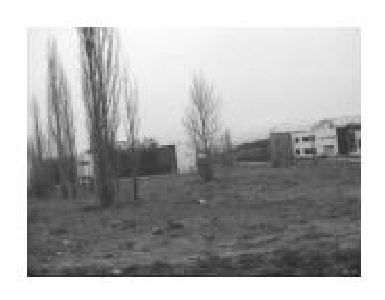
\includegraphics[width = 5cm]{./pictures/normale}}
	\end{subfigure}
	\begin{subfigure}[]
		{\label{fig:defocusNormaleFourier} 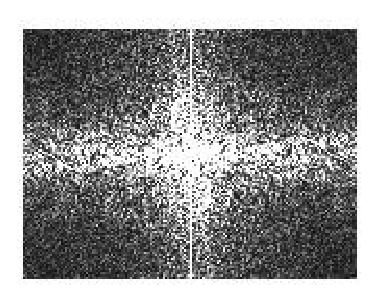
\includegraphics[width = 5cm]{./pictures/normale-fourier}}
	\end{subfigure}
	\begin{subfigure}[]
		{\label{fig:defocusSfocato} 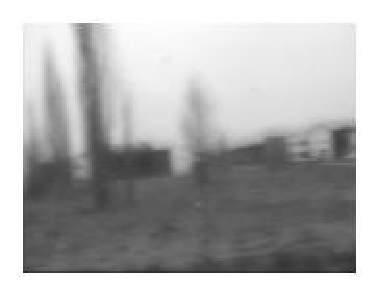
\includegraphics[width = 5cm]{./pictures/sfocato}}
	\end{subfigure}
	\begin{subfigure}[]
		{\label{fig:defocusSfocatoFourier} 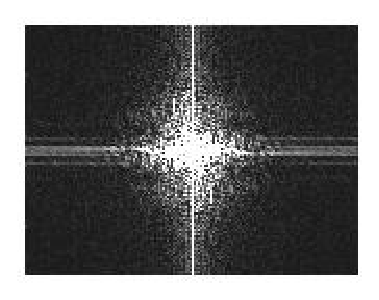
\includegraphics[width = 5cm]{./pictures/sfocato-fourier}}
	\end{subfigure}
	\caption{Comportamento della trasformata di Fourier nel caso di sfocatura}
	\label{fig:fourier}
\end{figure}
Nella figura \ref{fig:fourier} vediamo un esempio di come si comporta la trasformata di Fourier nel caso di sfocature: 
nel passaggio da un frame nitido (Fig. \ref{fig:defocusNormale}) a uno sfocato (Fig. \ref{fig:defocusSfocato}) abbiamo un crollo delle componenti ad alta frequenza nelle trasformate di Fourier (rispettivamente Fig. \ref{fig:defocusNormaleFourier} e Fig. \ref{fig:defocusSfocatoFourier}).
L'evento di tampering viene individuato quando l'\textit{energia media} della trasformata di Fourier (o di quella wavelet) del frame corrente $E_{HF}(z_i)$ \`e $Th$ volte minore di quella del background $E_{HF}(B_i)$:
\[E_{HF}(z_i)\leq Th E_{HF}(B_i),\]
dove $0<Th<1$ \`e  un valore di soglia scelto in base alla sensibilit\`a che si vuole dare all'algoritmo.\\
Un altro approccio consiste nell'analizzare la perdita di dettagli confrontando i contorni (\textit{edges}) del frame corrente con quelli del background.
Questo metodo, utilizzato in \cite{ellwart2012camera}, \cite{gil2007automatic}, \cite{harasse2004automated} e \cite{kryjak2012fpga}, consiste nell'estrarre i contorni dalle immagini secondo il metodo di Sobel \cite{sobel19683x3} o di Canny \cite{canny1986computational}, e confrontare il numero di pixel dei contorni con quelli del background. 
Quando il numero di pixel dei contorni del frame corrente $\sum edges(z_i)$ \`e $Th$ volte pi\`u piccolo di quello del background $\sum edges(B_i)$:
\[ \sum edges(z_i) \leq Th \sum edges(B_i), \]
dove $0<Th<1$ \`e  un valore di soglia scelto in base alla sensibilit\`a che si vuole dare all'algoritmo.
\subsection{Tecniche basate su monitoraggio sequenziale}
Le tecniche viste finora, come \`e stato detto nel paragrafo precedente, permettono di aggiornare ciascun frame con un modello della scena che viene calcolato in base alle osservazioni precedenti.
\begin{figure}
	\centering
	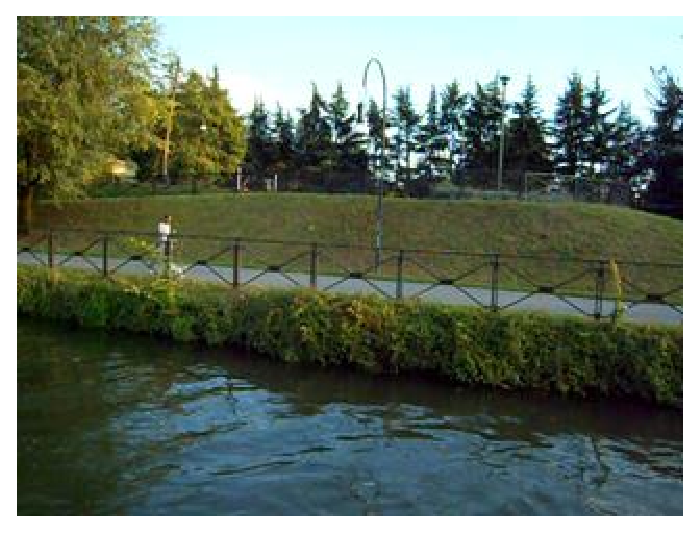
\includegraphics[width = 4cm]{./pictures/FPSalto/img0001}
	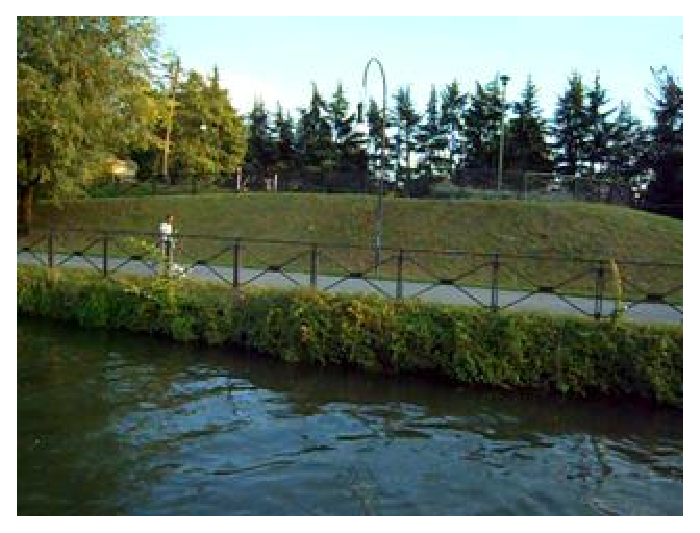
\includegraphics[width = 4cm]{./pictures/FPSalto/img0002}
	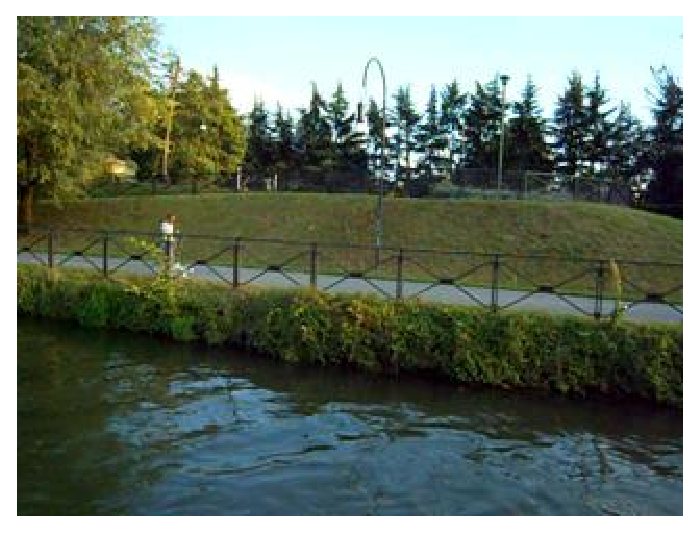
\includegraphics[width = 4cm]{./pictures/FPSalto/img0003}
	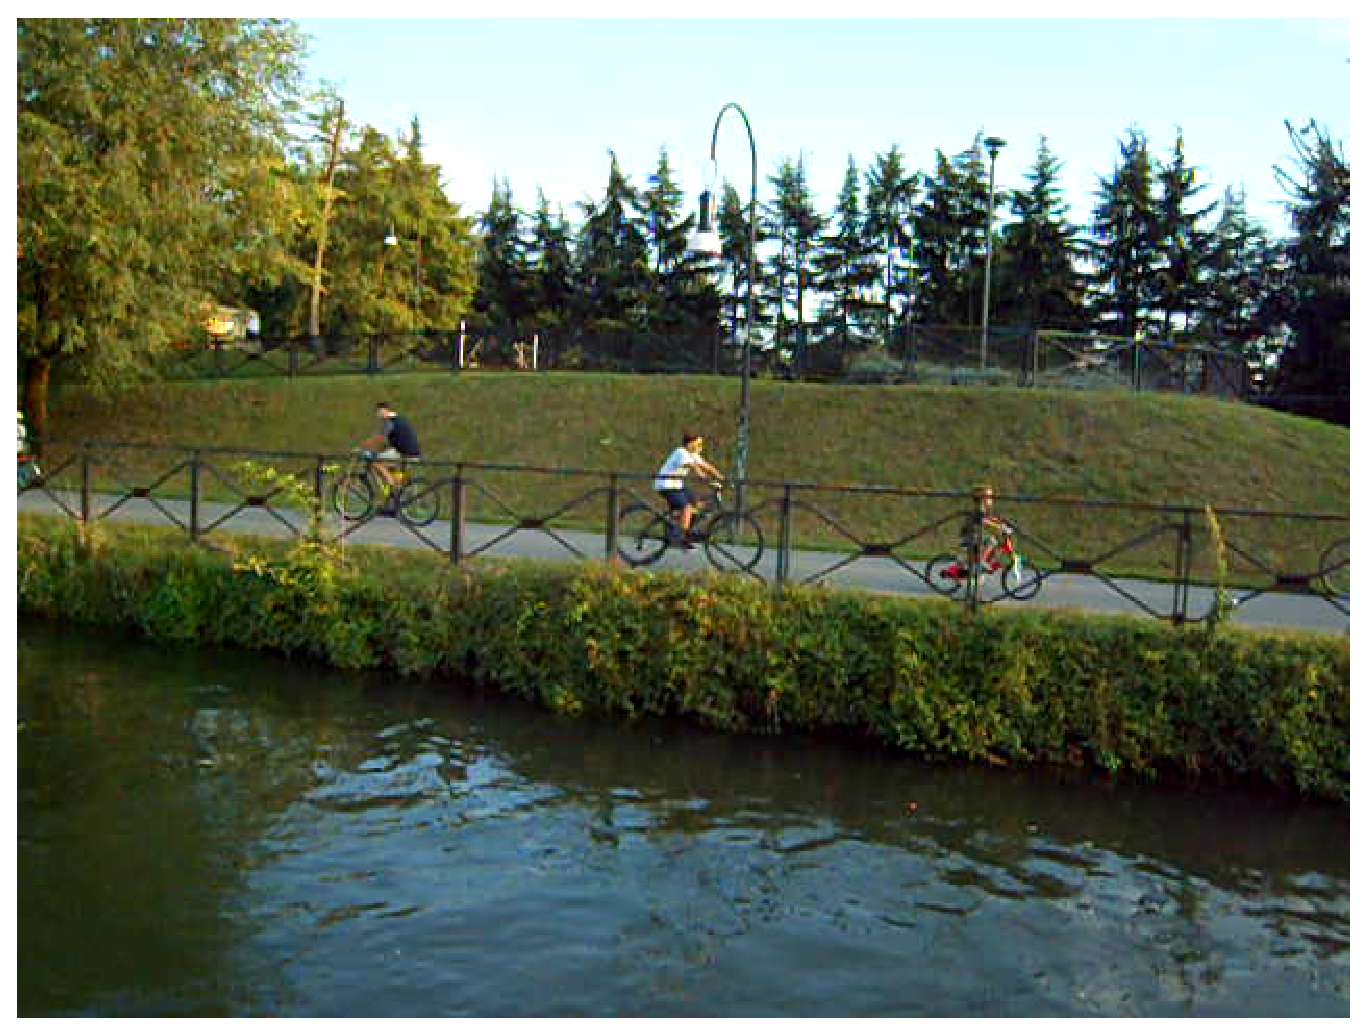
\includegraphics[width = 4cm]{./pictures/FPSalto/img0004}
	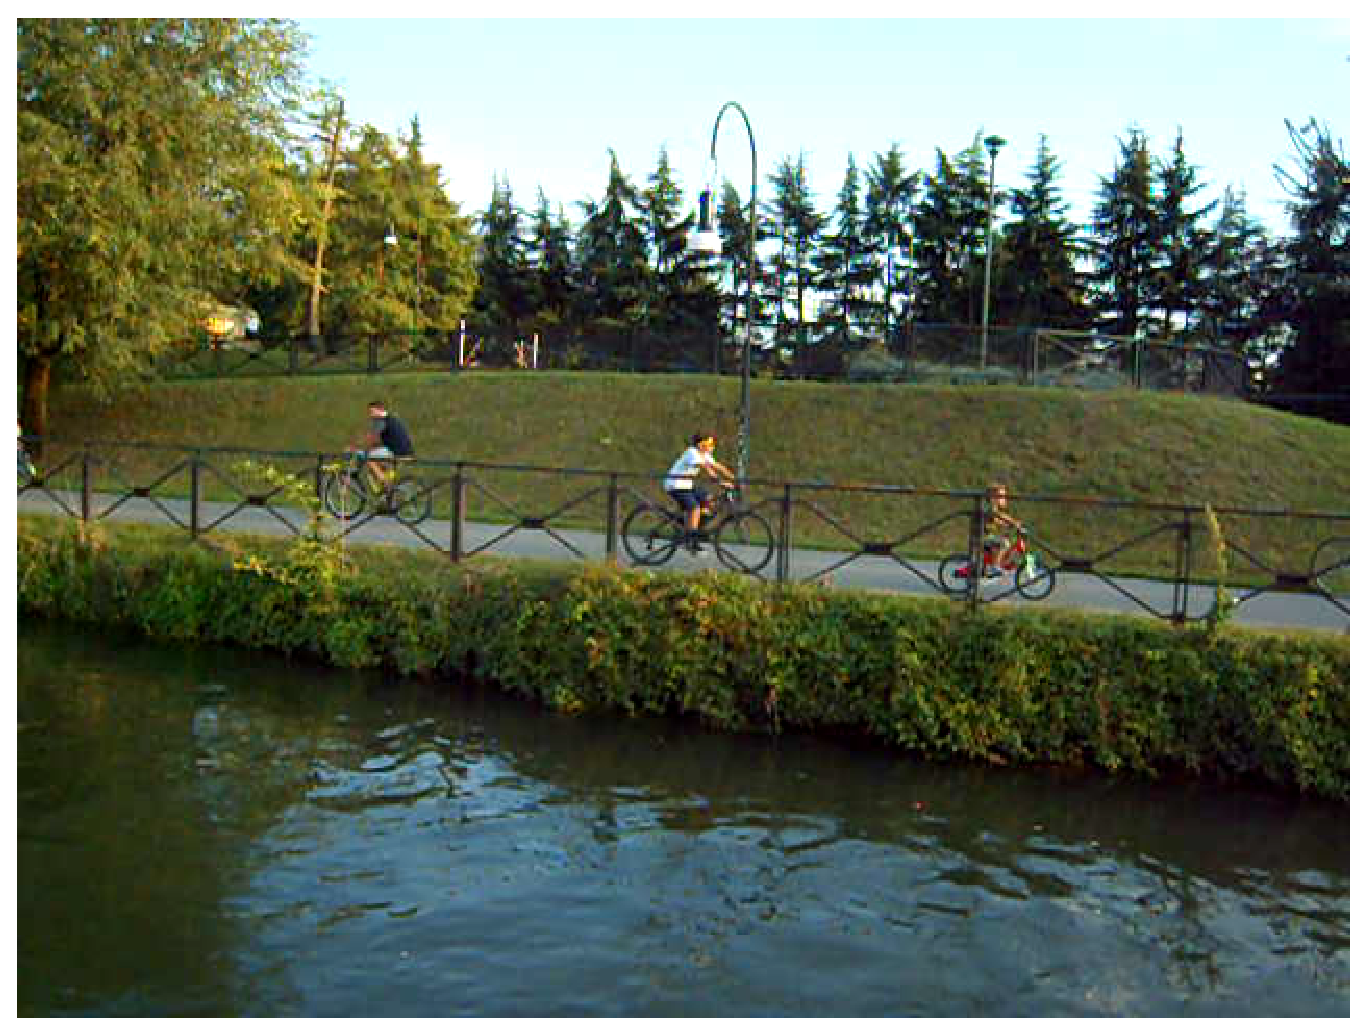
\includegraphics[width = 4cm]{./pictures/FPSalto/img0005}
	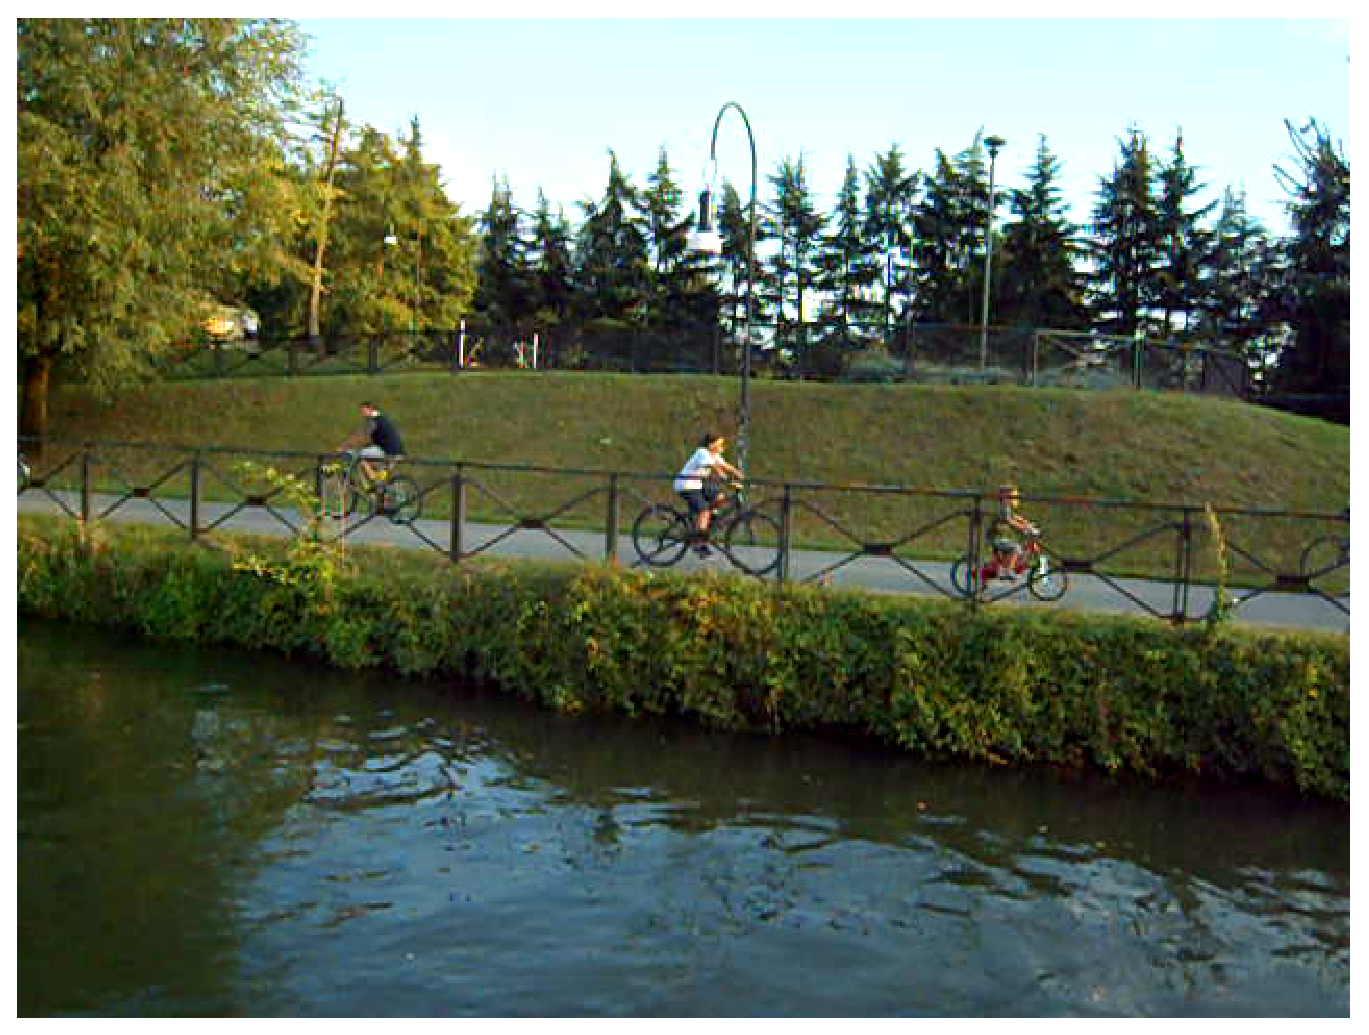
\includegraphics[width = 4cm]{./pictures/FPSalto/img0006}
	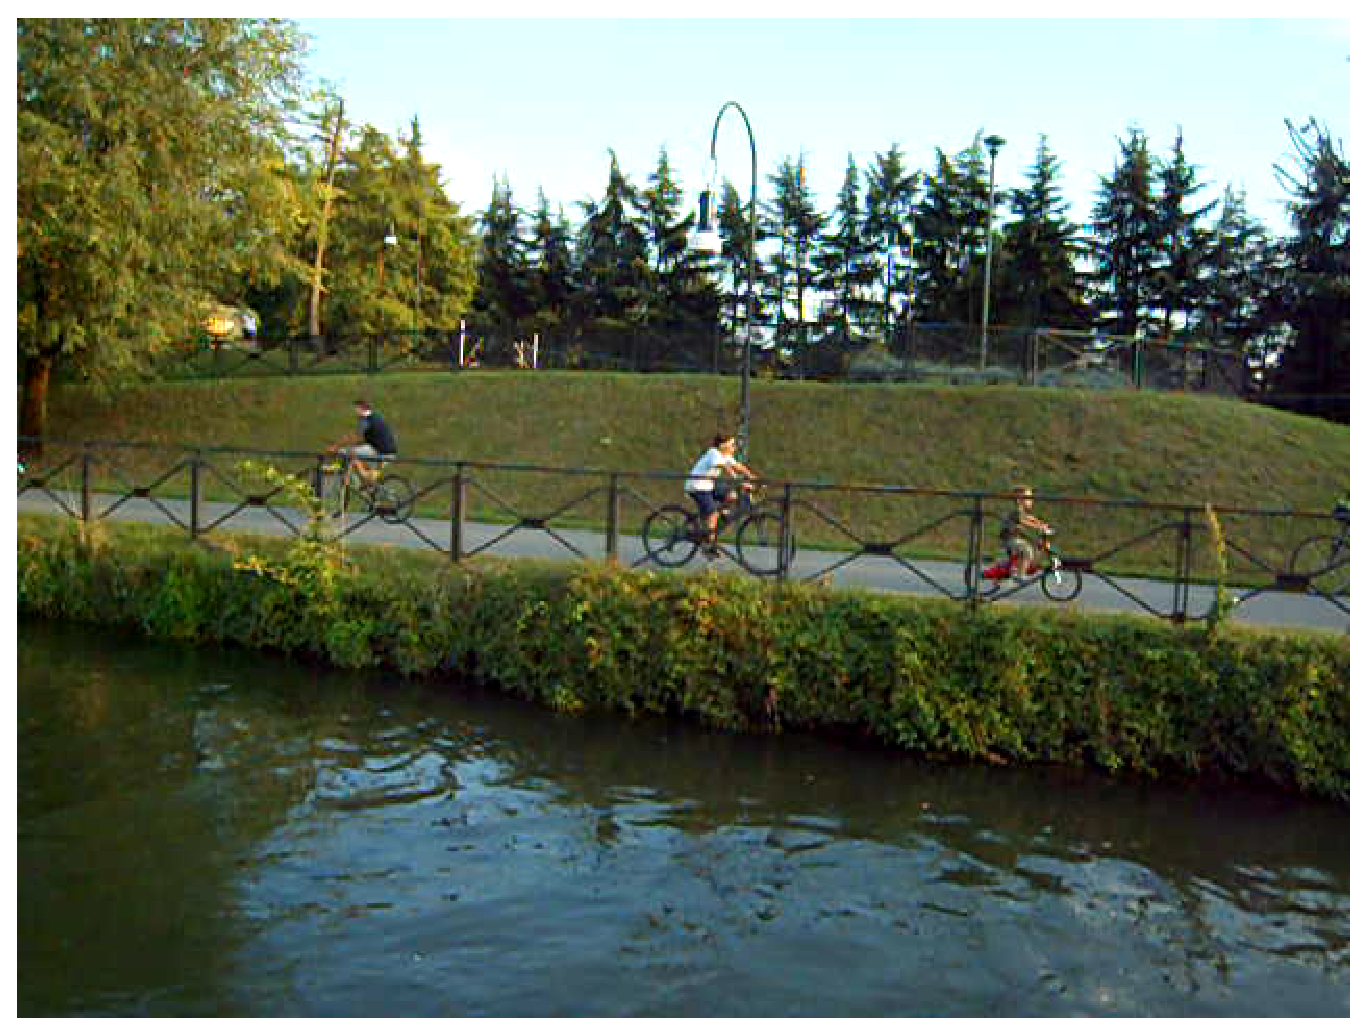
\includegraphics[width = 4cm]{./pictures/FPSalto/img0007}
	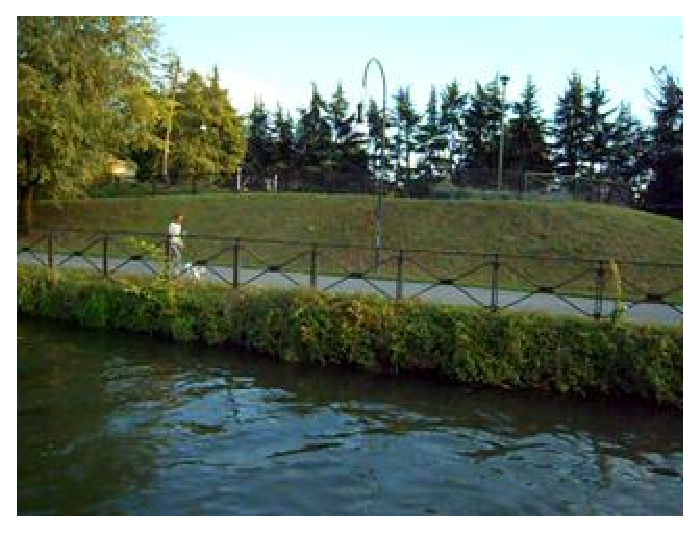
\includegraphics[width = 4cm]{./pictures/FPSalto/img0008}
	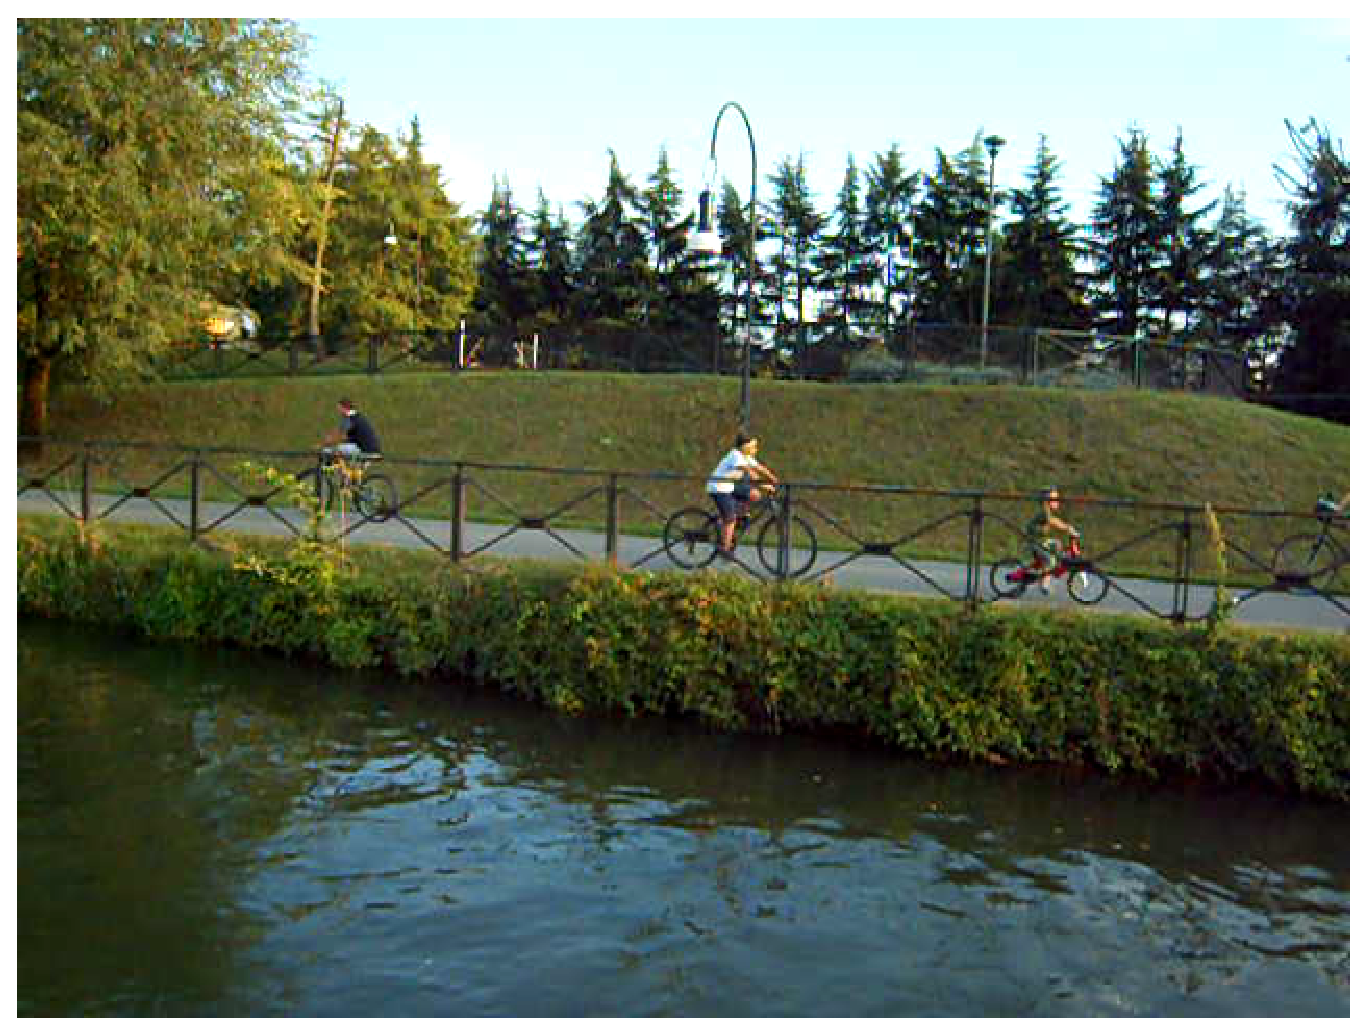
\includegraphics[width = 4cm]{./pictures/FPSalto/img0009}
	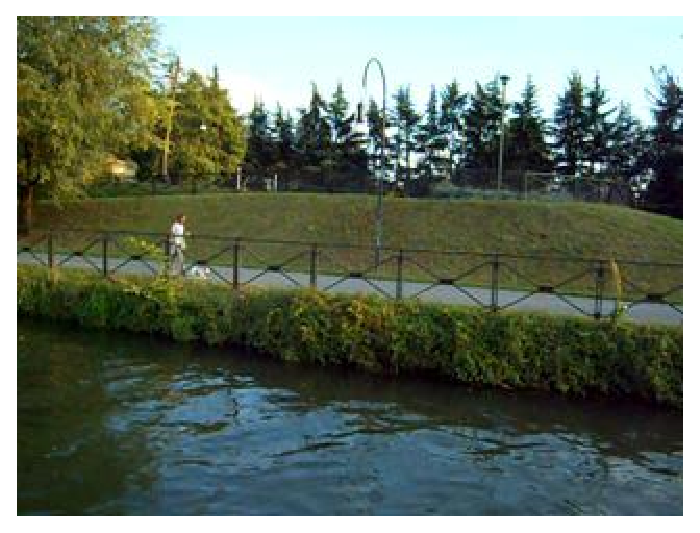
\includegraphics[width = 4cm]{./pictures/FPSalto/img0010}
	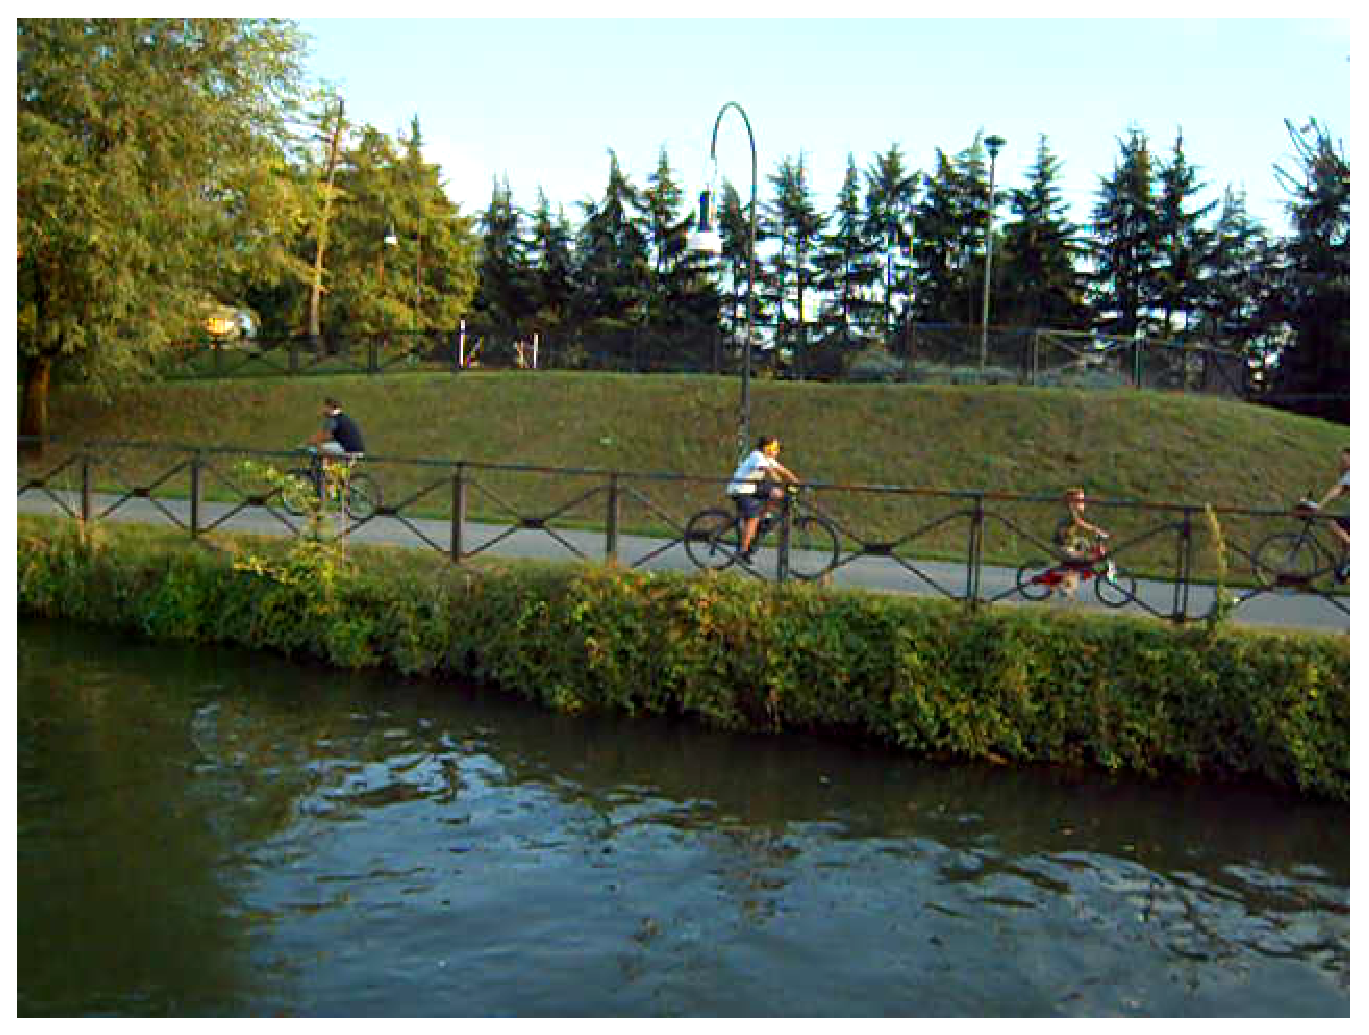
\includegraphics[width = 4cm]{./pictures/FPSalto/img0011}
	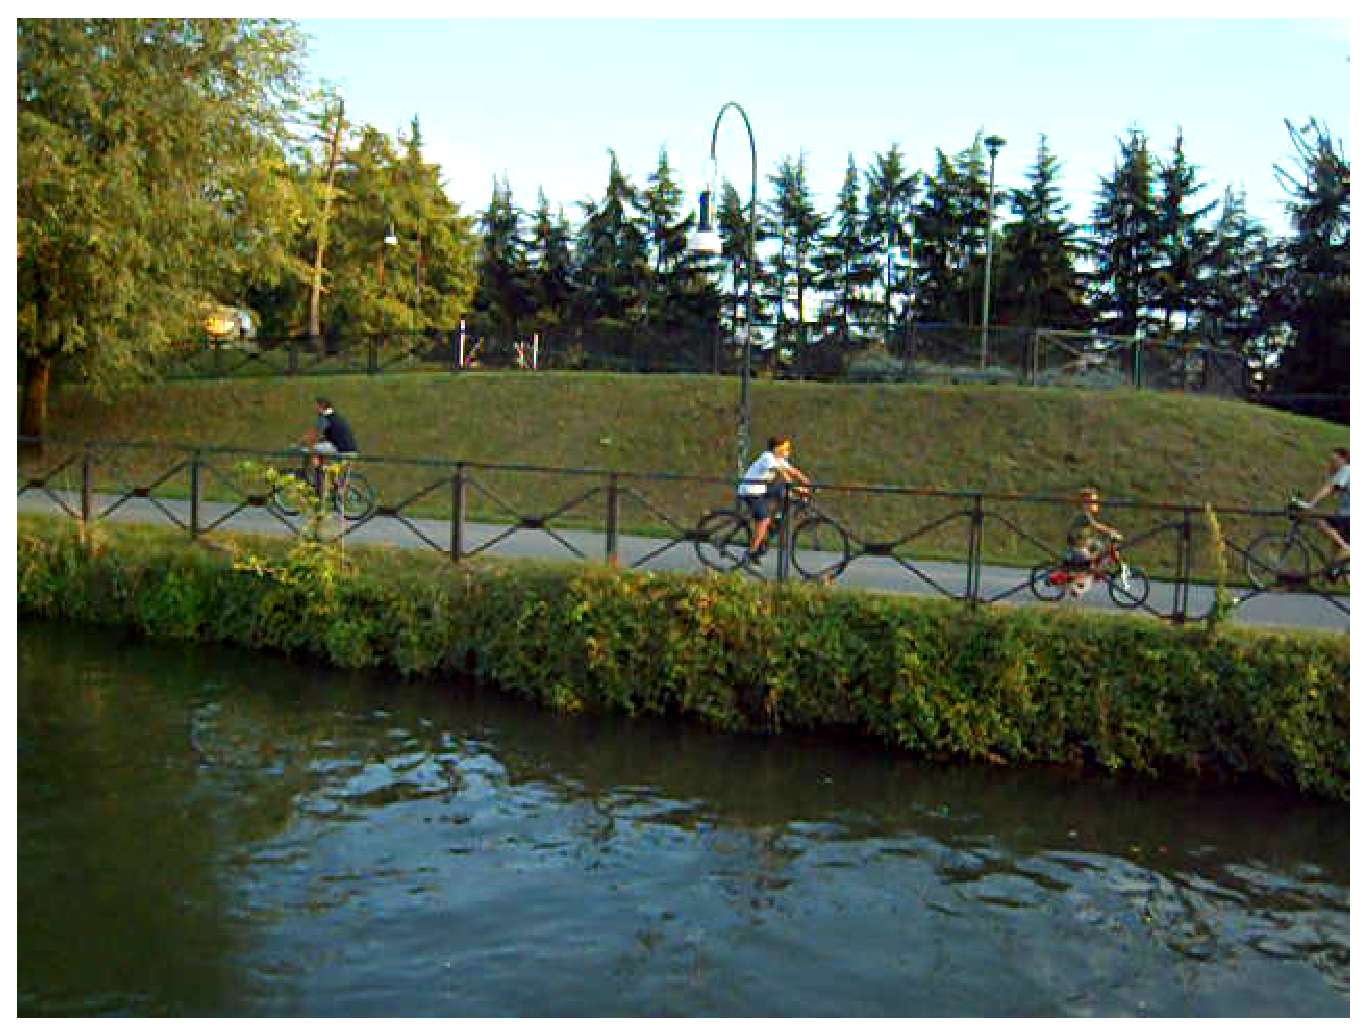
\includegraphics[width = 4cm]{./pictures/FPSalto/img0012}
	\caption{Sequenza di frame acquisiti a 30 fps}
	\label{fig:acquisizioneContinua}
\end{figure}
Questo approccio risulta fattibile nel caso in cui la camera operi con un framerate \textit{continuo}, solitamente tra i 30 frame per secondo (\textit{fps}) e i 2 fps. 
In questi casi, infatti, possiamo considerare che, tra un frame e il successivo, non avvengano grandi cambiamenti all'interno della scena e non cambi eccessivamente la luminosit\`a media.
La figura \ref{fig:acquisizioneContinua} mostra come, in un'acquisizione fatta a 30 fps, le differenze tra frame consecutivi siano quasi inesistenti. 
Un evento di tampering pu\`o, quindi, essere identificato in maniera molto semplice, in quanto una differenza molto elevata tra il frame analizzato e il background pu\`o essere dovuto solamente a un evento di tampering sulla camera.
La figura \ref{fig:acquisizioneBassa} mostra, invece, un esempio di frame acquisiti ogni 30 secondi.
Notiamo come le differenze tra immagini consecutive, in questo caso, siano pi\`u marcate rispetto al caso dell'acquisizione continua. 
\begin{figure}
	\centering
	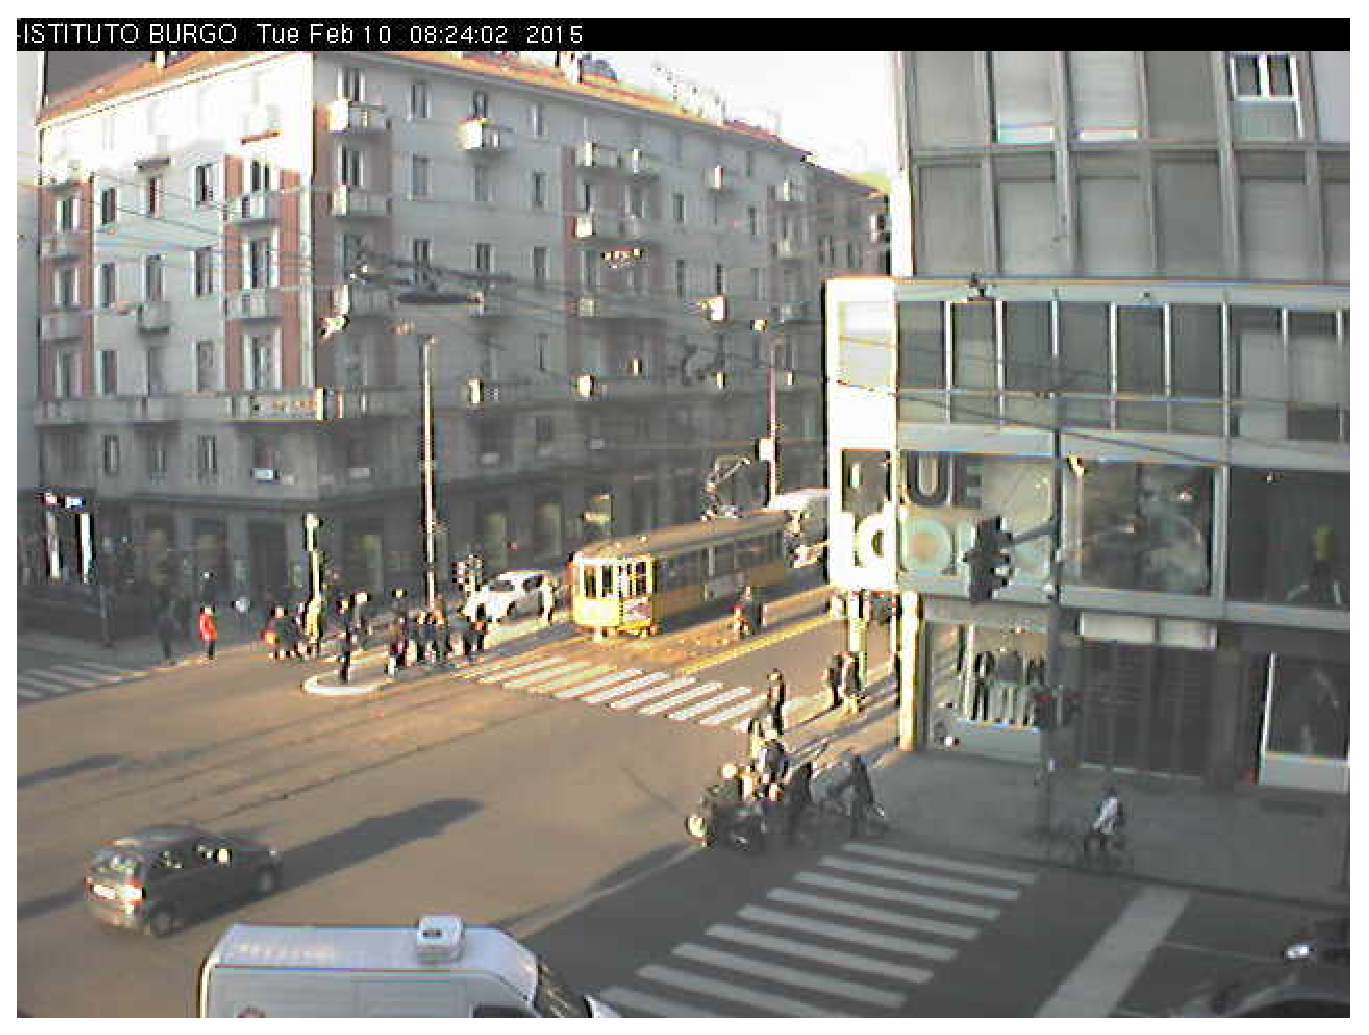
\includegraphics[width = 4cm]{./pictures/FPSbasso/image2691}
	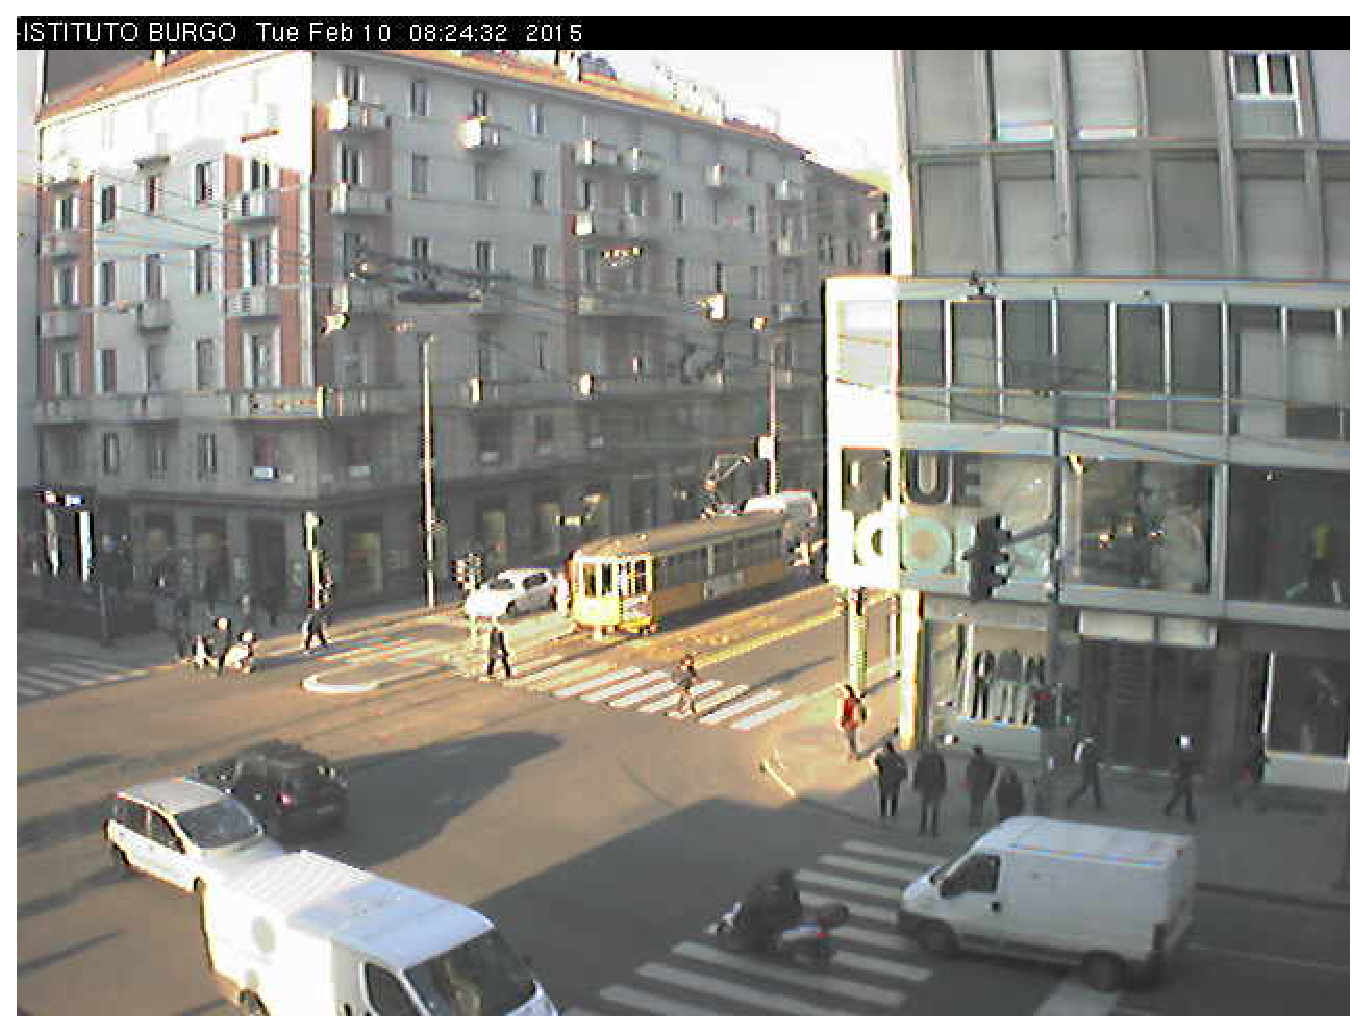
\includegraphics[width = 4cm]{./pictures/FPSbasso/image2692}
	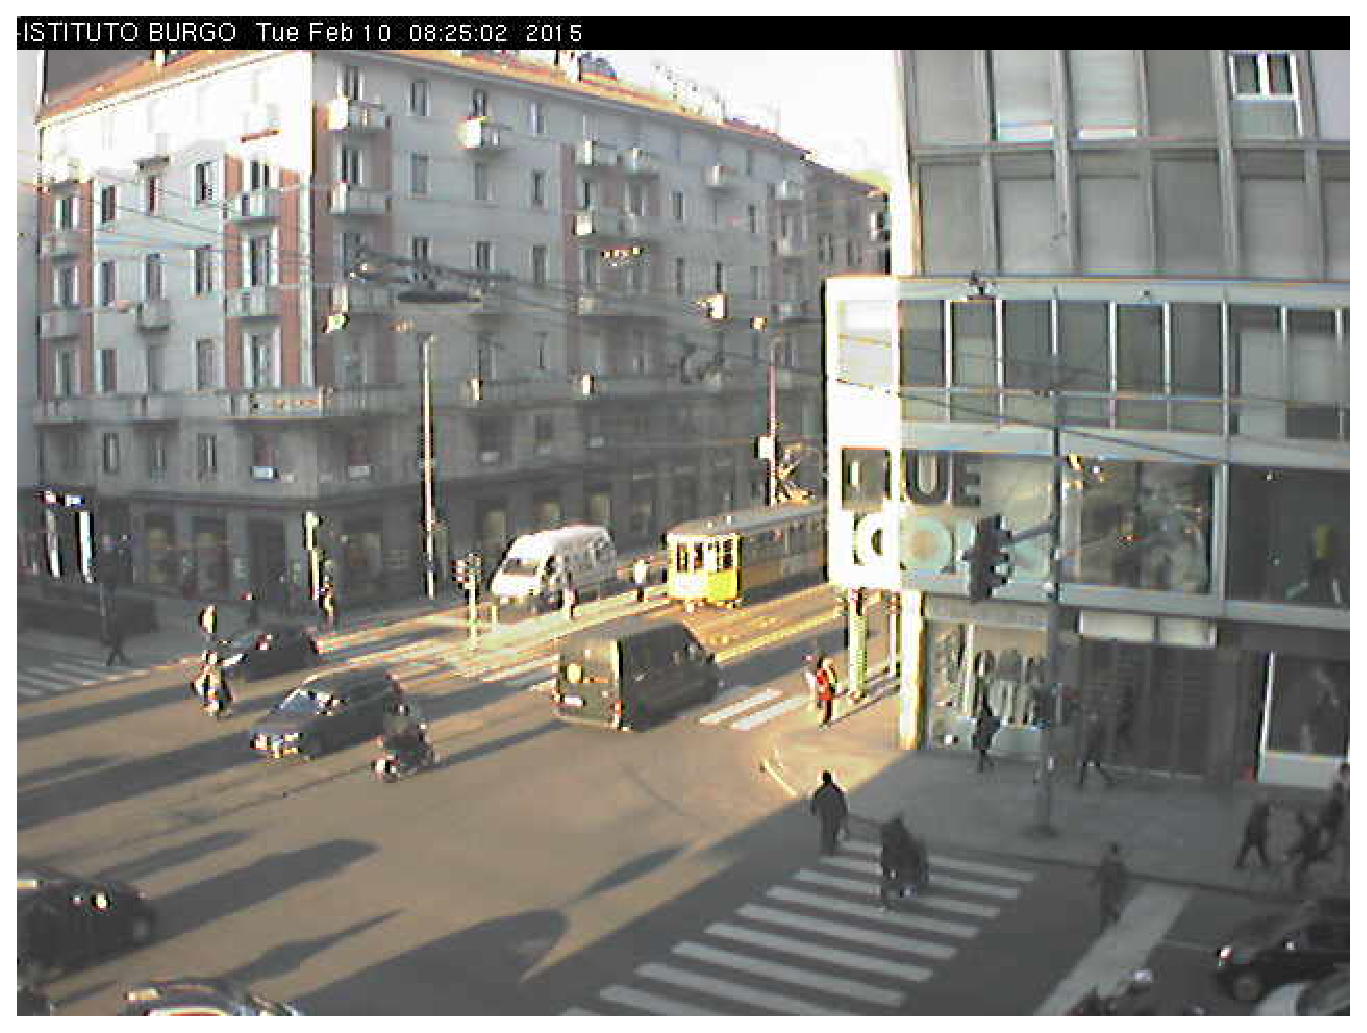
\includegraphics[width = 4cm]{./pictures/FPSbasso/image2693}
	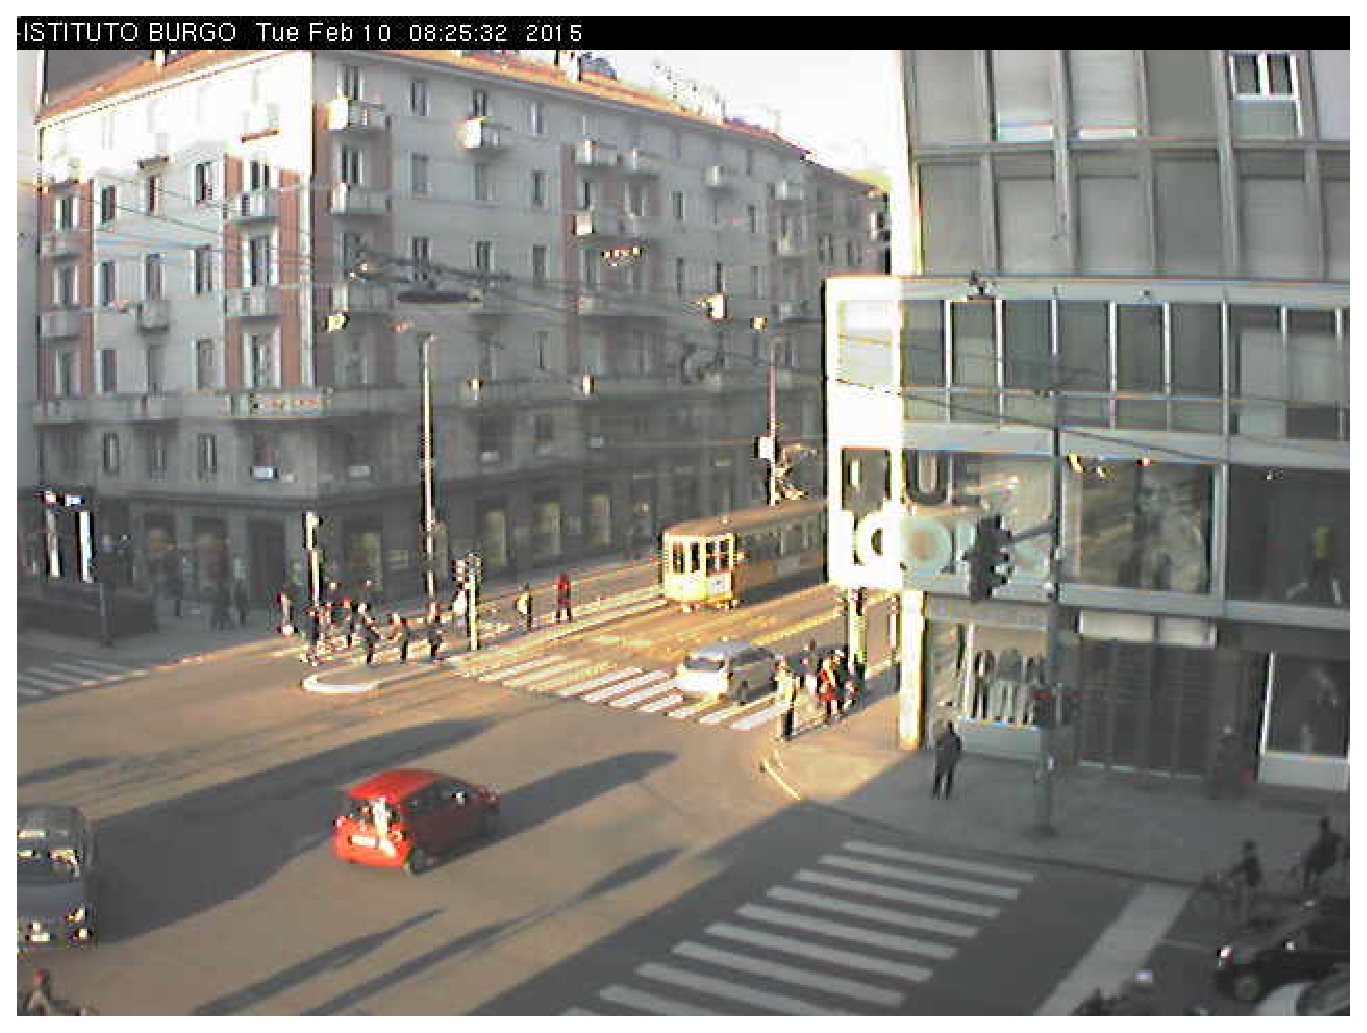
\includegraphics[width = 4cm]{./pictures/FPSbasso/image2694}
	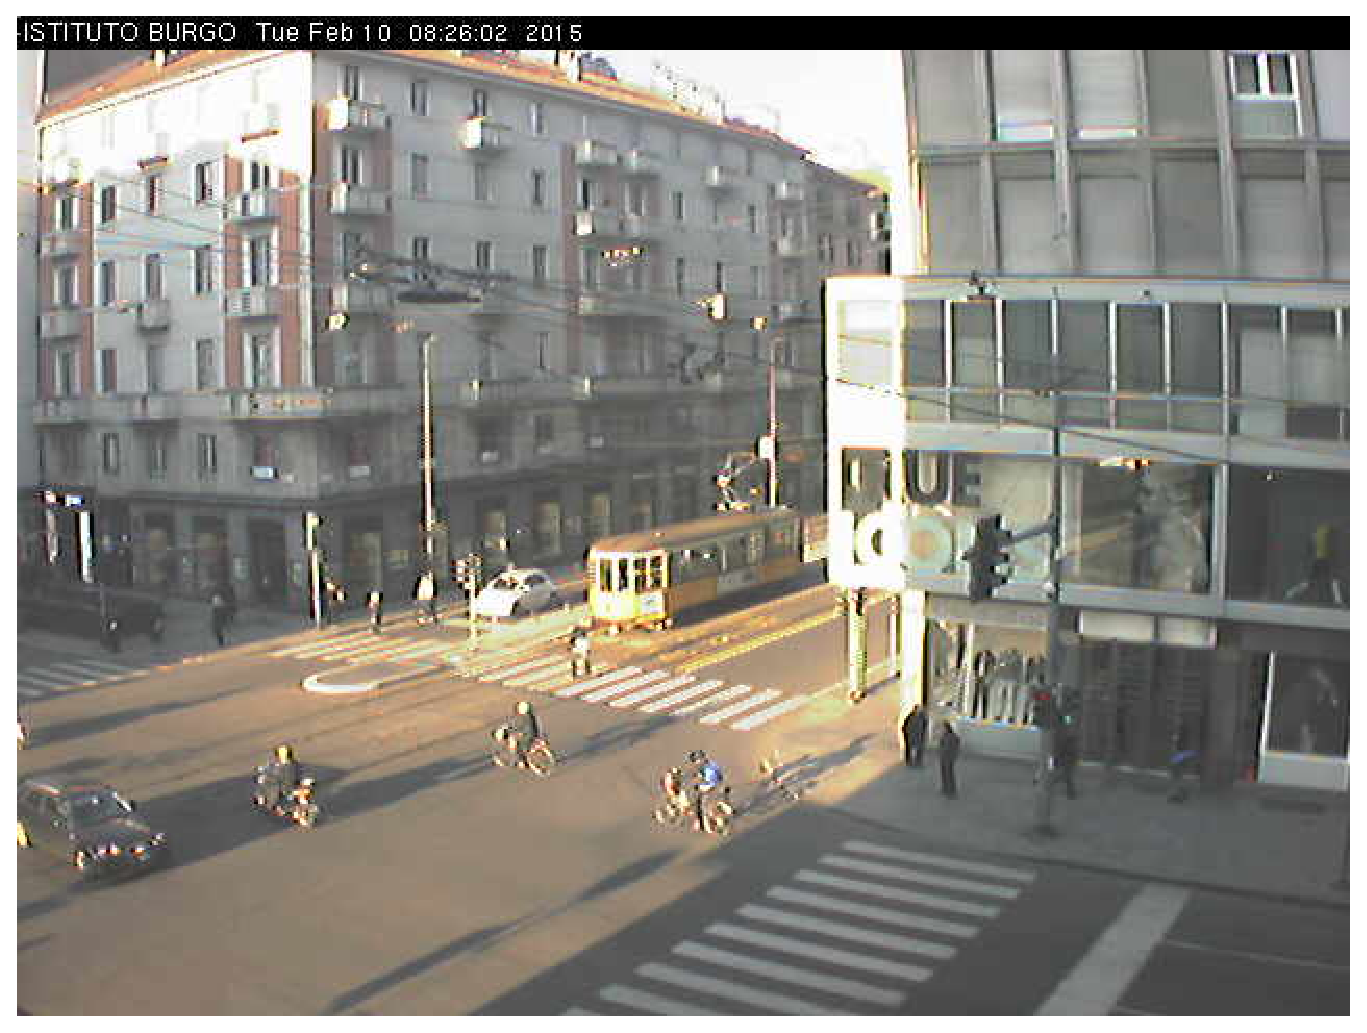
\includegraphics[width = 4cm]{./pictures/FPSbasso/image2695}
	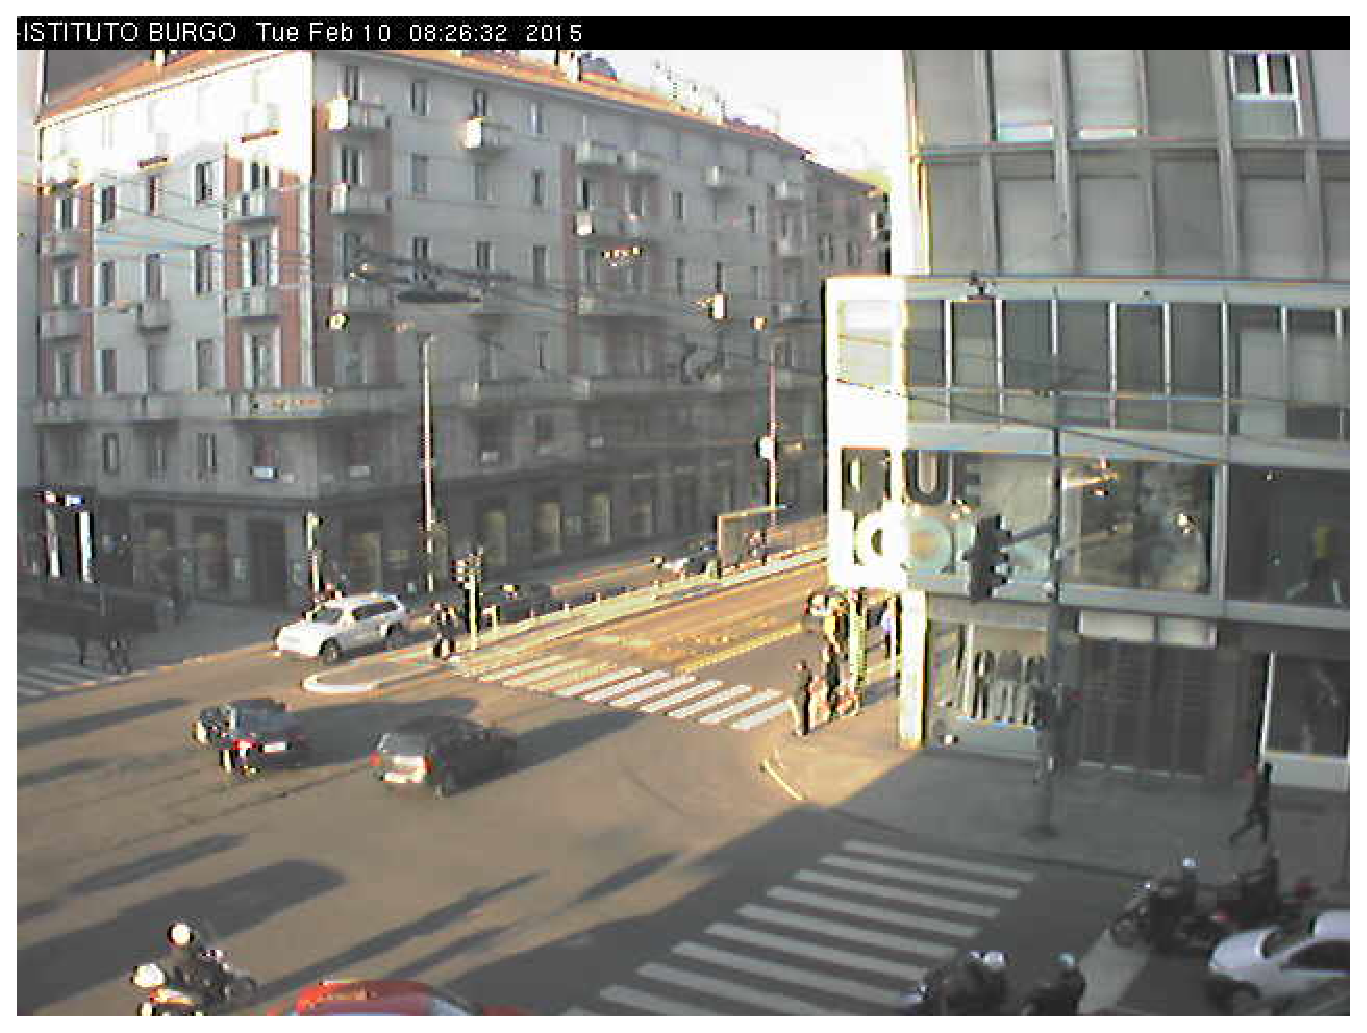
\includegraphics[width = 4cm]{./pictures/FPSbasso/image2696}
	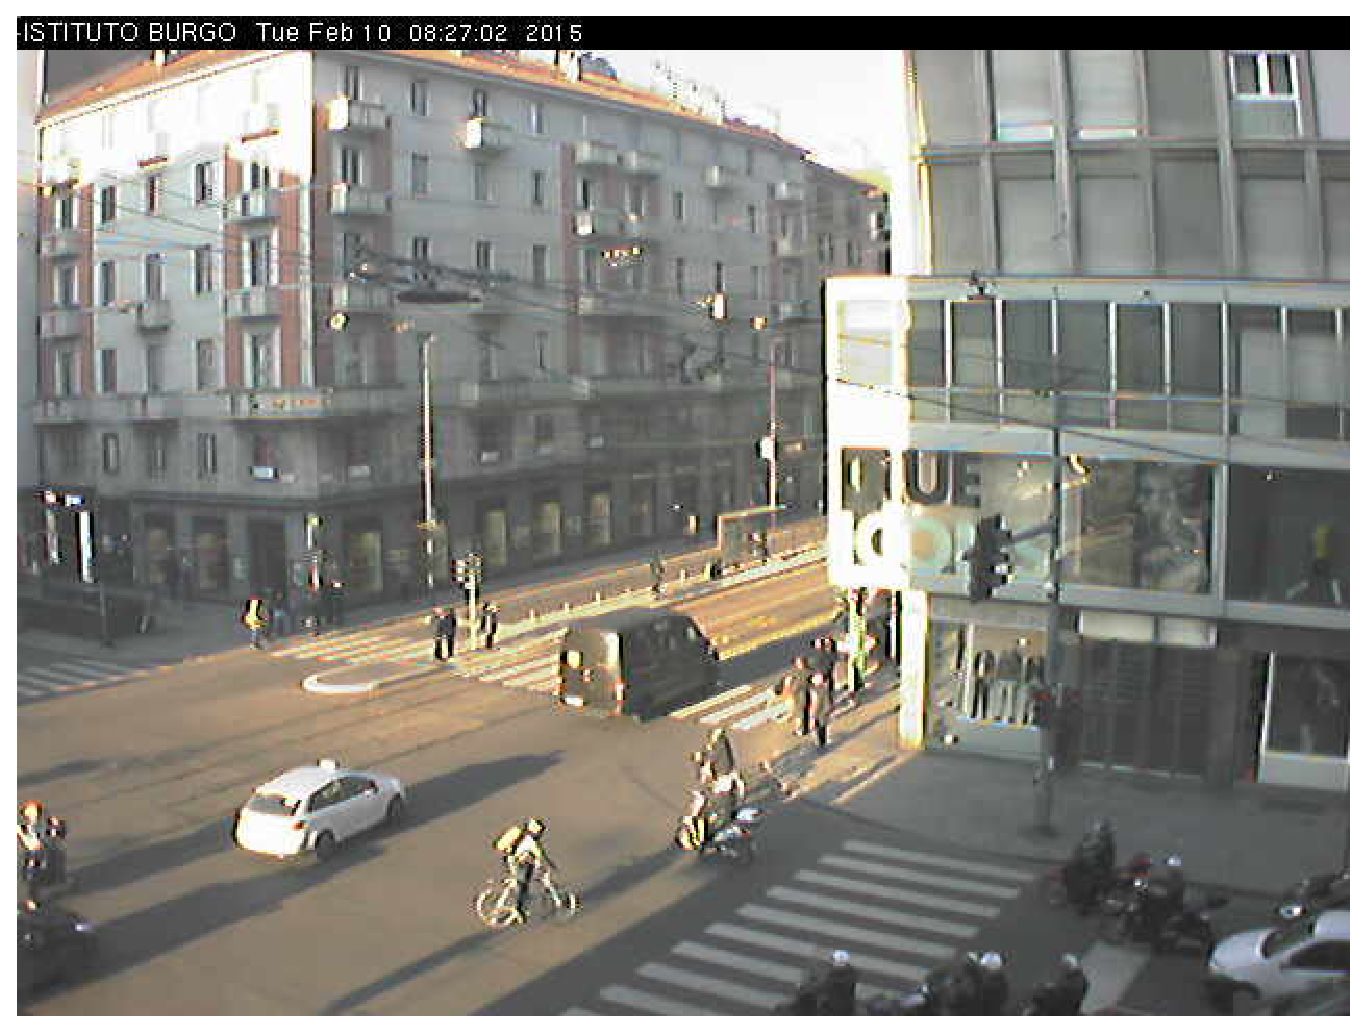
\includegraphics[width = 4cm]{./pictures/FPSbasso/image2697}
	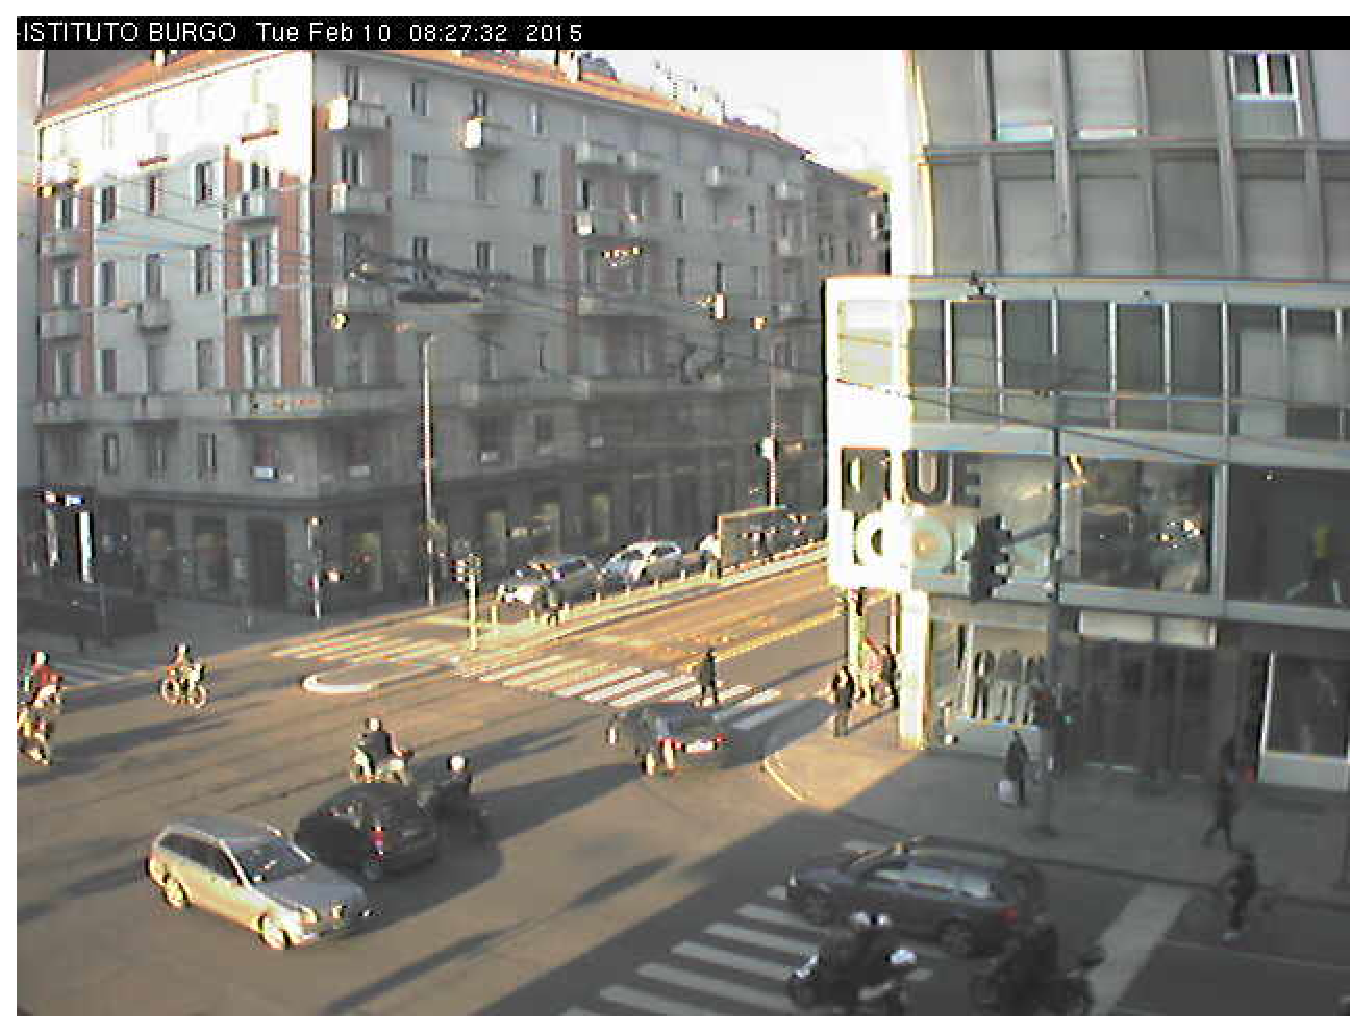
\includegraphics[width = 4cm]{./pictures/FPSbasso/image2698}
	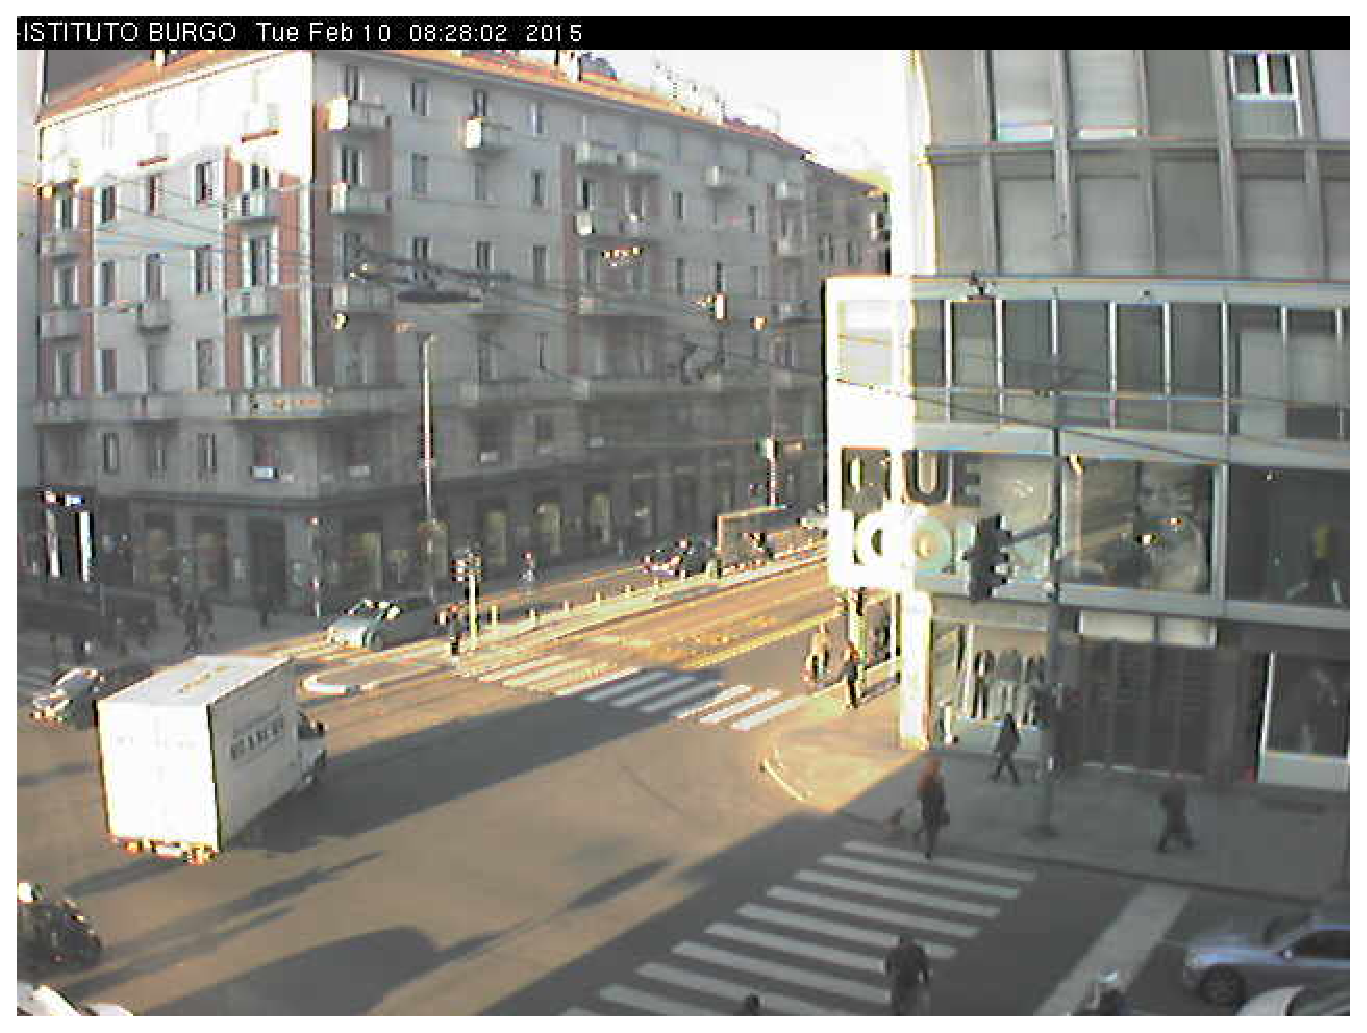
\includegraphics[width = 4cm]{./pictures/FPSbasso/image2699}
	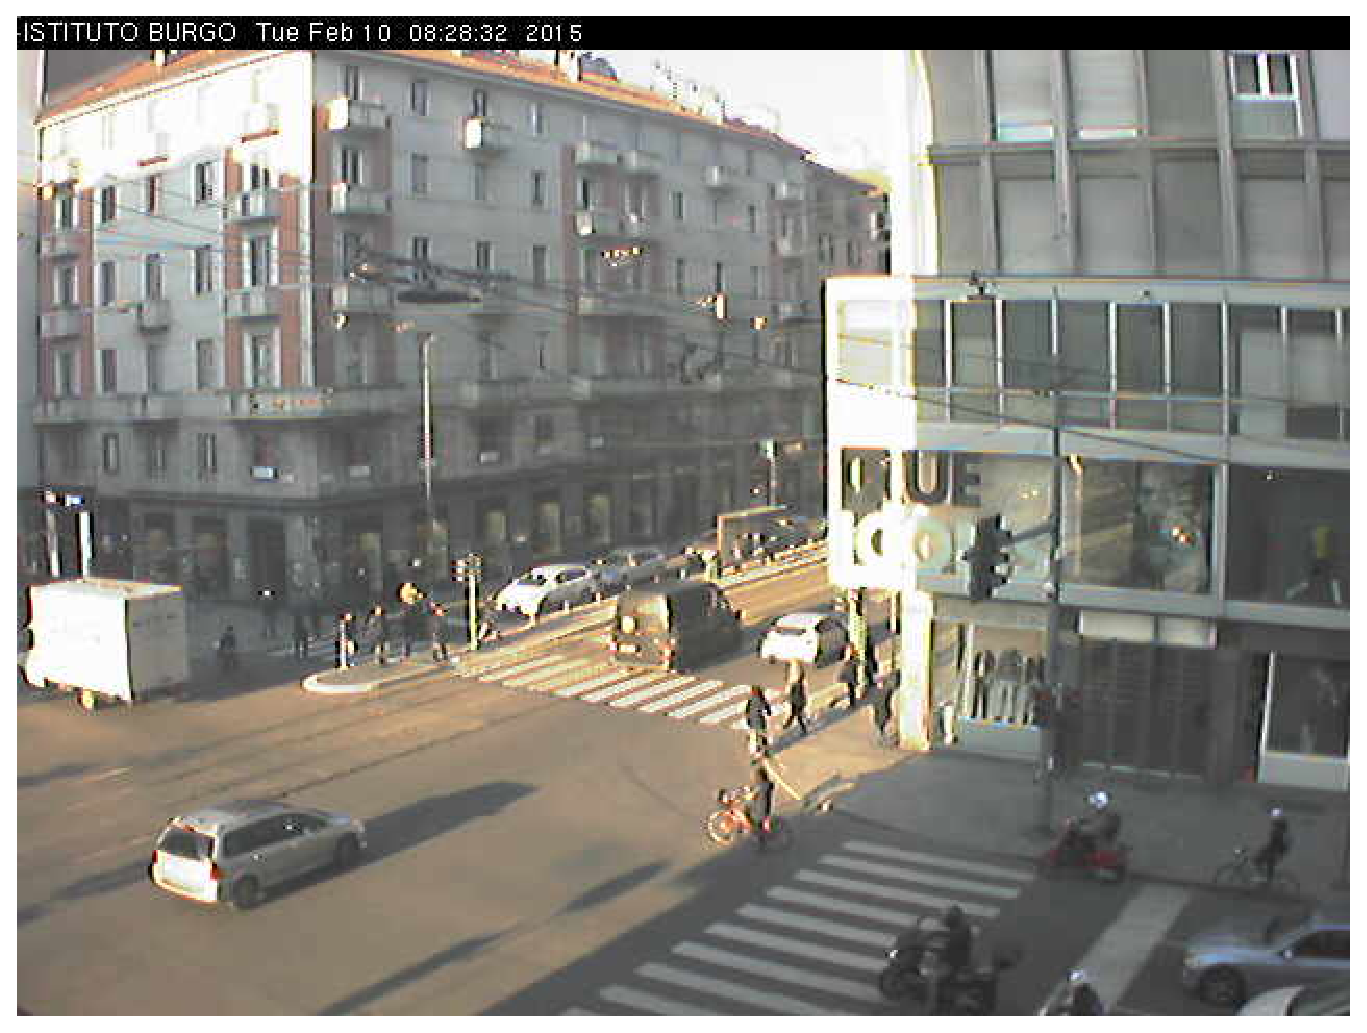
\includegraphics[width = 4cm]{./pictures/FPSbasso/image2700}
	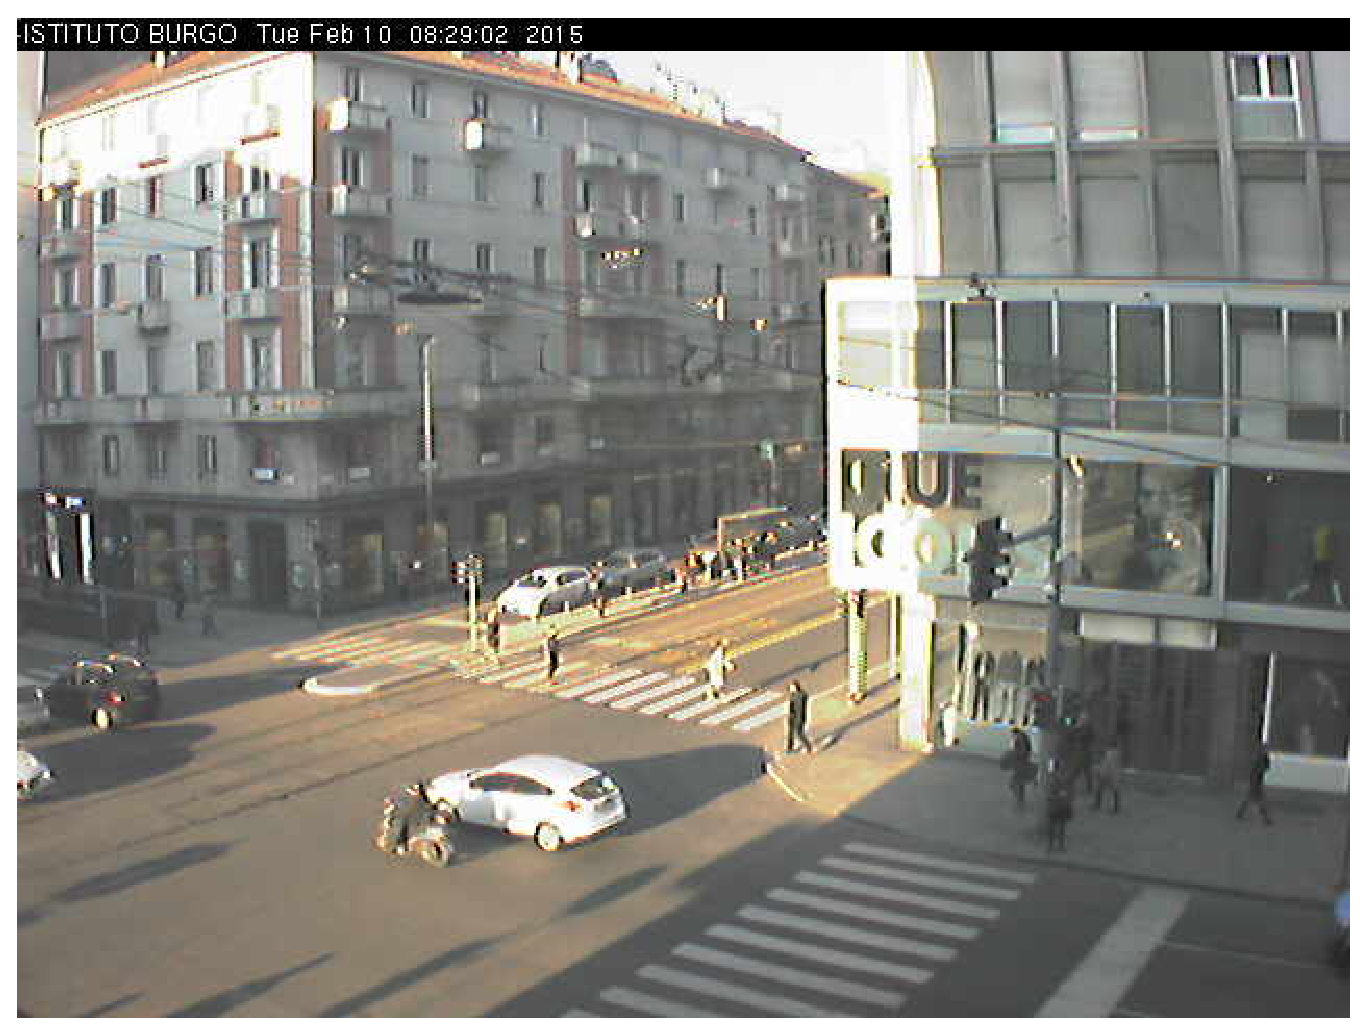
\includegraphics[width = 4cm]{./pictures/FPSbasso/image2701}
	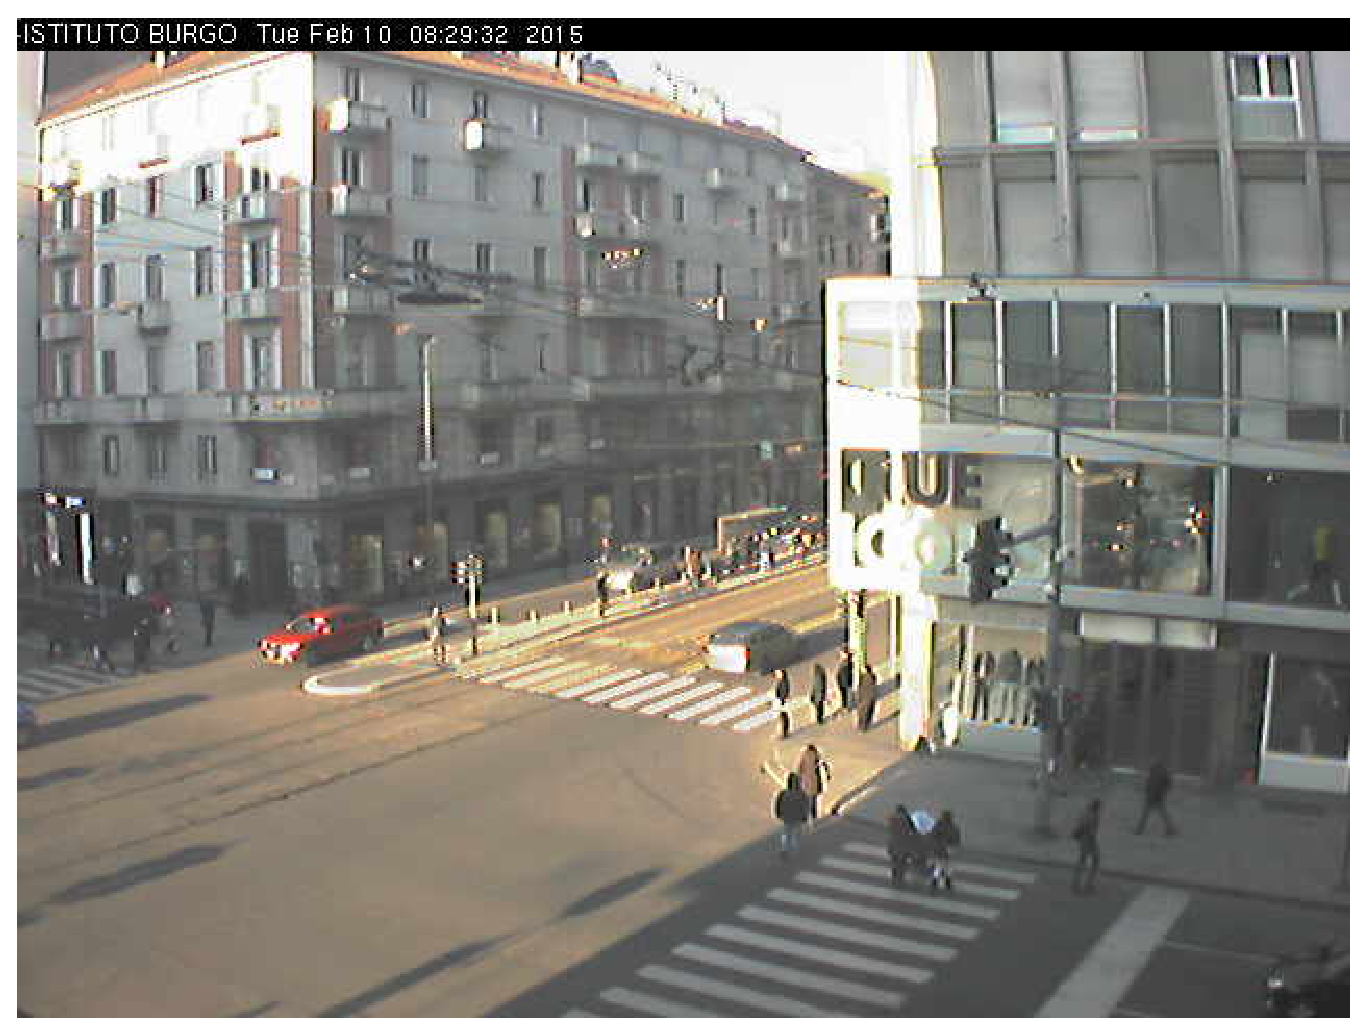
\includegraphics[width = 4cm]{./pictures/FPSbasso/image2702}
	\caption{Sequenza di frame acquisiti ogni 30 secondi}
	\label{fig:acquisizioneBassa}
\end{figure}
Questo fa s\`i che l'utilizzo di un modello di background risulti inefficiente.
Evidenziamo, inoltre, che le tecniche viste finora richiedono che il sistema di monitoraggio possegga elevate capacit\`a computazionali, in quanto l'aggiornamento del background e l'analisi di tampering detection non pu\`o rallentare la frequenza di acquisizione.\\
Un approccio alternativo consiste nel monitorare nel tempo il comportamento di alcuni indicatori estratti dalle singole immagini acquisite.
Si presuppone che, quando il sistema di monitoraggio opera in condizioni di funzionamento \textit{ottimali}, gli indicatori analizzati presentino una certa \textit{stazionariet\`a}, ovvero siano considerati dei campioni \textit{indipendenti} tra loro e distribuiti secondo una stessa funzione di ripartizione.
L'evento di tampering viene considerato come un \textit{cambiamento nella stazionariet\`a} di questi indicatori.\\
Il monitoraggio pu\`o avvenire utilizzando tecniche statistiche, come ad esempio \textit{change-point method} (CPM) \cite{ross2011nonparametric} o \textit{change-detection test} \cite{pimentel2014review}.
Troviamo alcuni esempi nell'identificazione di sfocature: in \cite{tsesmelis2013tamper} la soluzione consiste nel monitorare nel tempo il \textit{numero di SURF} \cite{bay2006surf}, in quanto tali descrittori decrementano in maniera considerevole il loro numero in presenza di sfocature.
Notiamo, per\`o, che l'utilizzo di una tecnica del genere richiede un elevato numero di calcoli per ricavare le SURF.
Il metodo, quindi, si presta poco a essere utilizzato su sistemi di monitoraggio a basso consumo.
Un altro esempio \`e dato da \cite{alippi2010detecting}, dove le sfocature vengono identificate monitorando l'\textit{energia media del gradiente} delle immagini acquisite:
\begin{equation}
\label{eq:energyGradient}
m_i = \mathcal{M}[z_i] = \int_{\mathcal{X}}\| \bigtriangledown z_i(x) \| _1 dx,
\end{equation}  
dove $\| \cdot \|_1$ si riferisce alla \textit{norma} $\mathcal{L}^1$. 
Per identificare il cambio di stazionariet\`a di questo indicatore vengono utilizzate tecniche di CDT basate su \textit{somme cumulate} (CUSUM) \cite{alippi2008just}.\\
Il test statistico utilizzato non richiede alcuna informazione \textit{a priori} del processo che si sta monitorando, e sfrutta una sequenza iniziale $\{m_i\}, i=1,\dots,T$ di indicatori estratti da frame non sfocati, in modo da configurare automaticamente i suoi parametri. 
Tale sequenza prende il nome di \textit{training set}, e permette di stimare la \textit{densit\`a probabilistica} (\textit{probability density function} (pdf)) di $m_i$ in assenza di sfocature, (i.e. l'\textit{ipotesi nulla}, indicata con $\Theta^0$), e di definire le \textit{ipotesi alternative}, indicate con $\Theta^1$, che identificano qualsiasi cambiamento non stazionario.\\
Per garantire una stima accurata dei parametri, \cite{alippi2010detecting} consiglia di utilizzare un training set ampio, ad esempio $T > 400$.
Il test opera su \textit{sotto-sequenze} di misure $m_i$ (ad esempio da $20$ misure) e stima la transizione da $\Theta^0$ a $\Theta^1$ misurando la \textit{log-verosimiglianza} tra la pdf in assenza di sfocature e le pdf delle varie ipotesi alternative nella sotto-sequenza $\tau$, ovvero
\[ r(\tau) = \ln \frac{N_{\Theta^1}(\phi_{\tau})}{N_{\Theta^0}(\phi_{\tau})}, \]
dove $\phi_{\tau}$ \`e il valore medio della misura $m_i$ nella sotto-sequenza $\tau$, e $N_{\Theta}$ \`e la \textit{distribuzione gaussiana multivariata} parametrizzata in $\Theta$.\\
Il metodo CUSUM considera la \textit{somma cumulata} 
\[ S(\tau) = \sum^\tau_{t=1} r(t) \]
e identifica un cambiamento in $m_i$ quando \[g(\tau)=S(\tau)-\nu(\tau),\] ovvero la differenza tra il valore della somma cumulata all'istante $\tau$ e il suo valore minimo nel tempo \[\nu(\tau)=\min_{t=1,...,\tau}S(t),\] supera una certa soglia $h$.\\
L'utilizzo di una tecnica sequenziale per l'identificazione di sfocature permette di operare con una bassa complessit\`a computazionale, tanto da poter essere utilizzato come soluzione a livello di nodo per una \textit{wireless multimedia sensor network} (WMSN) \cite{akyildiz2007survey}.
D'altro canto, confrontato con le tecniche descritte nel paragrafo \ref{background}, questo metodo genera un numero pi\`u alto di \textit{falsi allarmi}, il che si traduce, all'interno di una rete di sensori, in un aumento dei messaggi di allarme inviati, che devono essere considerati, quindi, come un costo.